% 
% ---------------------------------------------------------------
% Copyright (C) 2012-2018 Gang Li
% ---------------------------------------------------------------
%
% This work is the default powerdot-tuliplab style test file and may be
% distributed and/or modified under the conditions of the LaTeX Project Public
% License, either version 1.3 of this license or (at your option) any later
% version. The latest version of this license is in
% http://www.latex-project.org/lppl.txt and version 1.3 or later is part of all
% distributions of LaTeX version 2003/12/01 or later.
%
% This work has the LPPL maintenance status "maintained".
%
% This Current Maintainer of this work is Gang Li.
%
%

\documentclass[
 size=12pt,
 paper=smartboard, %a4paper, smartboard, screen
 mode=present, %present, handout, print
 display=slides, % slidesnotes, notes, slides
% nohandoutpagebreaks,
% pauseslide,
style=tuliplab,
% nopagebreaks,clock
% hlentries=true,
% hlsections = true,
pauseslide,
fleqn,leqno]{powerdot}

\hypersetup{pdfpagemode=FullScreen}
% \usepackage[toc,highlight,blackslide,slidesonly,sounds,HA]{HA-prosper}

\usepackage{amssymb}
\usepackage{amsmath} 
\usepackage{rotating}
\usepackage{graphicx}
\usepackage{boxedminipage}
\usepackage{media9}
\usepackage{rotate}
\usepackage{calc}
\usepackage[absolute]{textpos}
\usepackage{psfrag,overpic}
\usepackage{fouriernc}
\usepackage{pstricks,pst-node,pst-text,pst-3d,pst-grad}
\usepackage{moreverb,epsfig,color,subfigure}
\usepackage{color}
\usepackage{pstricks}
\usepackage{pstricks-add}
\usepackage{pst-text}
\usepackage{pst-node, pst-tree}
\usepackage{booktabs}
\usepackage{etex}
\usepackage{breqn}
\usepackage{multirow}
\usepackage{gitinfo2}


\usepackage{listings}
\lstset{frameround=fttt, 
frame=trBL, 
stringstyle=\ttfamily,
backgroundcolor=\color{yellow!20},
basicstyle=\footnotesize\ttfamily}
\lstnewenvironment{code}{
\lstset{frame=single,escapeinside=`',
backgroundcolor=\color{yellow!20},
basicstyle=\footnotesize\ttfamily}
}{}


\usepackage{fouriernc}
\usepackage{hyperref}

%%%%%%%%%%%%%%%%%%%%%%%%%%%%%%%%%%%%%%%%%%%%%%%%%%%%%%%%%%%%%%%%%%%%%%%%
% title
% TODO: Customize to your Own Title, Name, Address
%
\title{New York City Taxi Trip Duration}
\author{
Gengwang Li
\\
Flip00 Final Presentation
% \href{mailto:gangli@acm.org}{gangli@acm.org}
% \and % more authors
}
\date{\gitCommitterDate}


% Customize the setting of slides
\pdsetup{
% theslide=\arabic{slide}~/~\pageref*{lastslide},
% theslide=\arabic{slide},
rf=\href{http://www.tulip.org.au}{
Last Changed by: \textsc{\gitCommitterName}\ v0.1-\gitDescribe\ (\gitAuthorDate)
},
cf=\hyperlink{blankslide}{Flip00 Final Presentation},
trans=Fade,
list={labelsep=1em,leftmargin=*,itemsep=0pt,topsep=5pt,parsep=0pt},
% counters={theorem,lemma},
% randomdots,dmaxdots=80
}


\begin{document}

\maketitle 

\begin{slide}[toc=,bm=]{Overview}
\tableofcontents[content=sections]
\end{slide}


\section{Introduction}

\begin{slide}[toc=,bm=]{Overview of the Introduction}
\tableofcontents[content=currentsection,type=0]
\end{slide}

\begin{slide}{Description of Competition}
  \begin{itemize}
    \item Description \pause
    \begin{itemize}
      \item Challenging to build a model that predicts the total ride duration of taxi trips in New York City.
    \end{itemize} \pause
    \item Given \pause
    \begin{itemize}
      \item Geographic positions of picking up and dropoffing;
      \item Timestamps of picking up and dropoffing;
      \item Number of passengers;
      \item Vendor id of the texi;
      \item and a flag indicates if the trip record was sent with delay
    \end{itemize} \pause
    \item Evaluation \pause
    \begin{itemize}
      \item The evaluation metric of this competition is Root Mean Squared Logarithmic Error.
      $$
      \epsilon = \sqrt{\frac{1}{n} \sum_{i=1}^{n}{(log(p_i + 1) - log(a_i + 1))^2}}
      $$ 
      \pause
      \item $\epsilon$ is the RMSLE value (score)
      \item $n$ is the total number of observations in the (public/private) data set,
      \item $p_i$ is your prediction of trip duration, and
      \item $a_i$ is the actual trip duration for . 
      \item $log$ is the natural logarithm of 
    \end{itemize} 
  \end{itemize}
\end{slide}

\begin{slide}{Dataset}
  \begin{itemize}
    \item Take a look at the files
      \begin{itemize}
        \item train.csv - the training set (contains 1458644 trip records)
        \item test.csv - the testing set (contains 625134 trip records)
        \item sample_submission.csv - a sample submission file in the correct format
      \end{itemize}
  \end{itemize}
  \pause
  \begin{figure}[h]
    \centering
    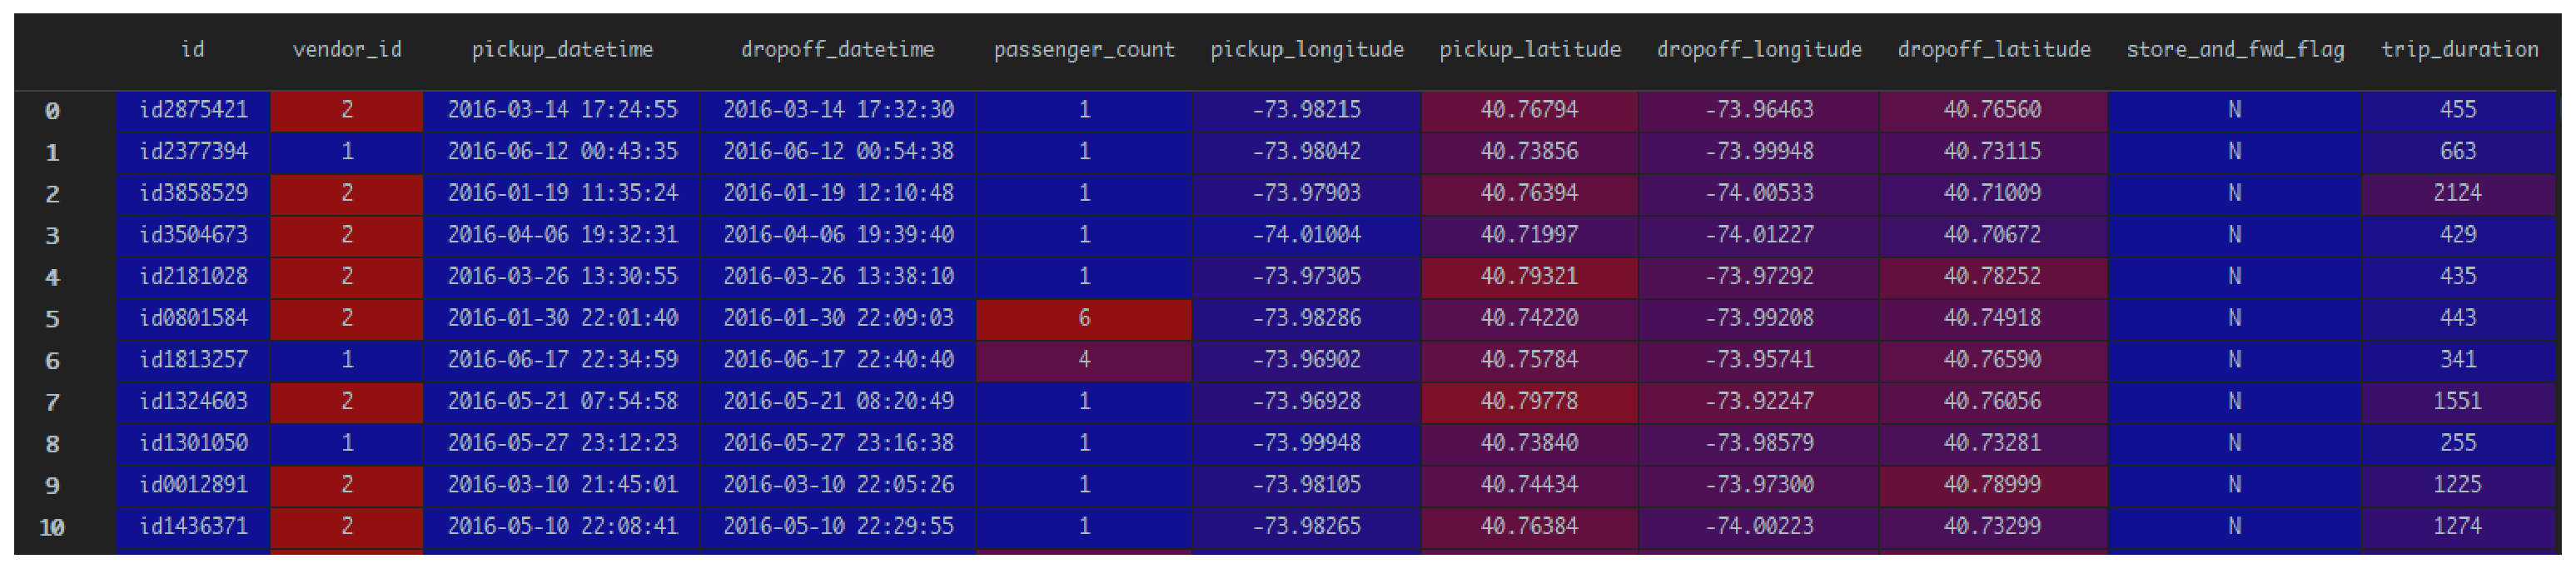
\includegraphics[width=1.0\textwidth]{figures2/train_data.eps}
    \caption{train dataset}
    \label{fig:train-dataset}
  \end{figure}
\end{slide}

\begin{slide}{Preview}
  \begin{itemize}
    \item Overview train and test dataset
  \end{itemize}
  \pause
  \begin{figure}[v]
    \begin{minipage}[t]{0.8\linewidth}
      \centering
      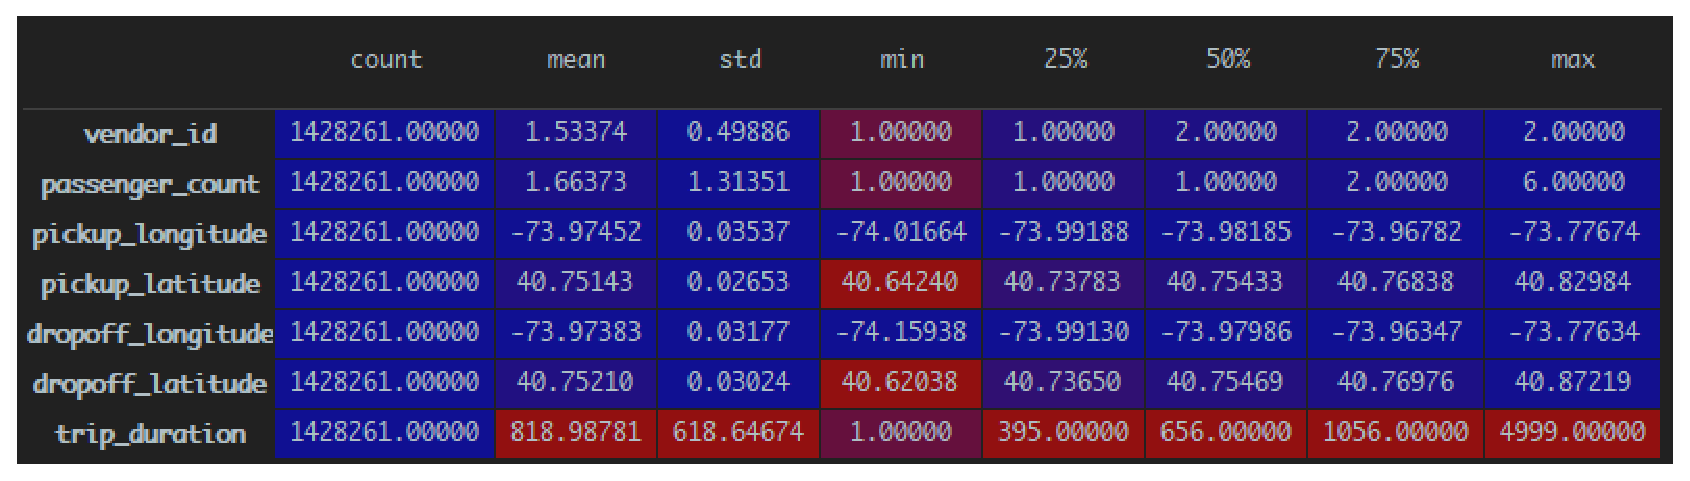
\includegraphics[width=1.0\textwidth]{figures2/train_data_desc.eps}
      \caption{Description of train dataset}
      \label{fig:categories-picture}
    \end{minipage} \pause
    \vfill 
    \begin{minipage}[t]{0.8\linewidth}
      \centering
      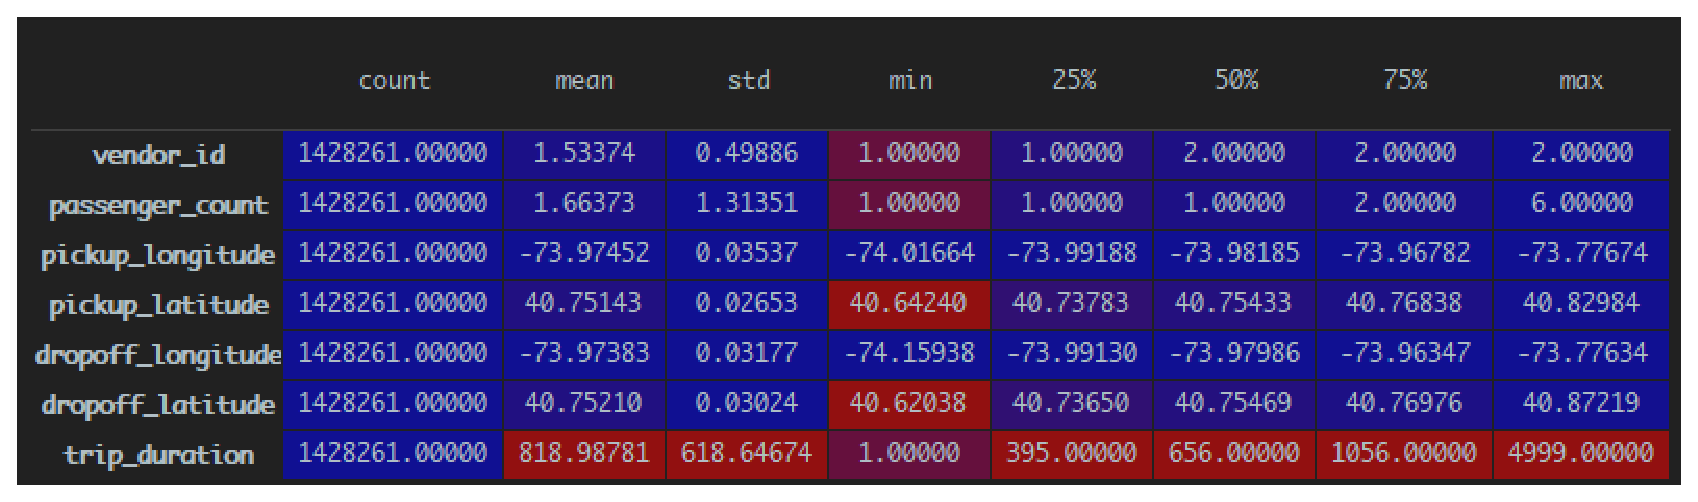
\includegraphics[width=1.0\textwidth]{figures2/test_data_desc.eps}
      \caption{Description of test dataset}
      \label{fig:pic-label1}
    \end{minipage}
  \end{figure}
\end{slide}

\begin{slide}{Missing values}
  \begin{itemize}
    \item Missing values?
  \end{itemize}
  \pause
  \begin{figure}[h]
    \centering
    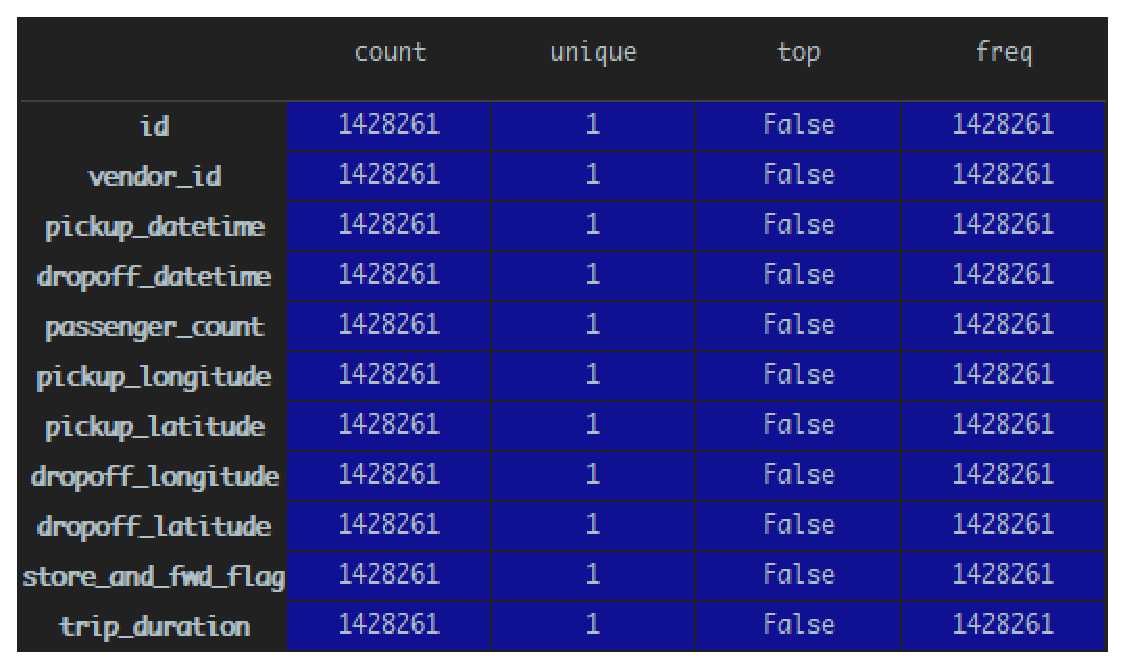
\includegraphics[width=0.6\textwidth]{figures2/train_null.eps}
    \caption{Statistics of missing value}
    \label{fig:missing-value-pic}
  \end{figure}
\end{slide}


\section{Visualization}

\begin{slide}[toc=,bm=]{Overview of Visualization}
  \tableofcontents[content=currentsection,type=0]
\end{slide}

\begin{slide}{Review Features}
  \begin{itemize}
    \item Review features \pause
    \begin{itemize}
      \item Vendor id of the texi; \pause
      \item Number of passengers; \pause
      \item Geographic positions of picking up and dropoffing; \pause
      \begin{itemize}
        \item pickup_longitude, pickup_latitude
        \item dropoff_longitude, dropoff_latitude
      \end{itemize} \pause
      \item Timestamps of picking up and dropoffing; \pause
      \begin{itemize}
        \item pickup_datetime
        \item dropoff_datetime
      \end{itemize} \pause
      \item A flag indicates if the trip record was sent with delay
    \end{itemize}
  \end{itemize}
\end{slide}

\begin{slide}{Geographic}
  \begin{itemize}
    \item Pickup vs dropoff positions
  \end{itemize}
  \begin{figure}[h]
    \centering
    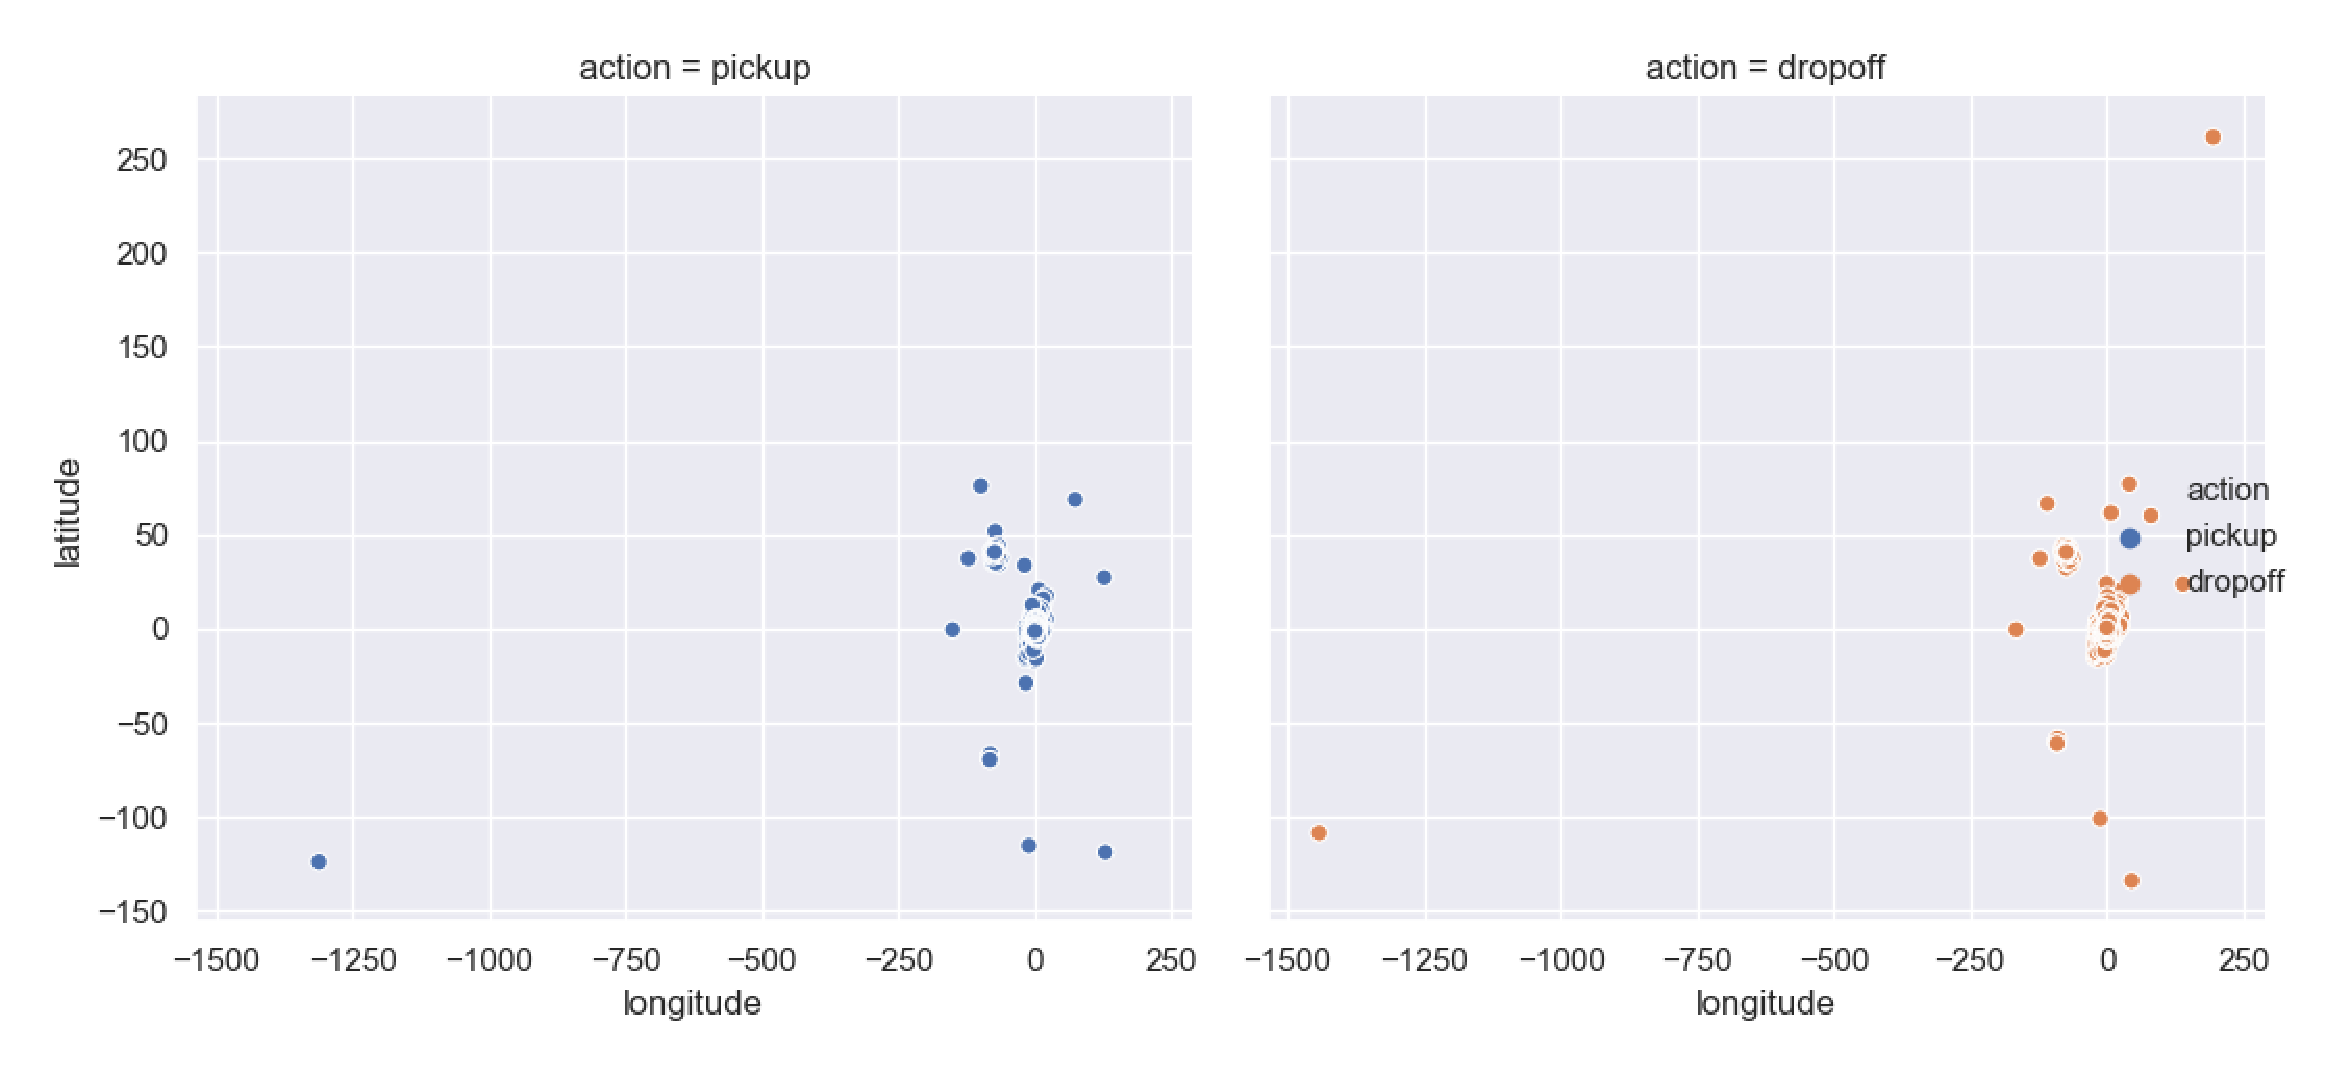
\includegraphics[width=0.8\textwidth]{figures2/action_geo.eps}
    \caption{Pickup vs dropoff locations plot}
    \label{fig:pickup-dropoff-position}
  \end{figure}
\end{slide}

\begin{slide}{Geographic-Duration}
  \begin{itemize}
    \item Faraway position has less relation with large duration 
  \end{itemize}
  \begin{figure}[h]
    \centering
    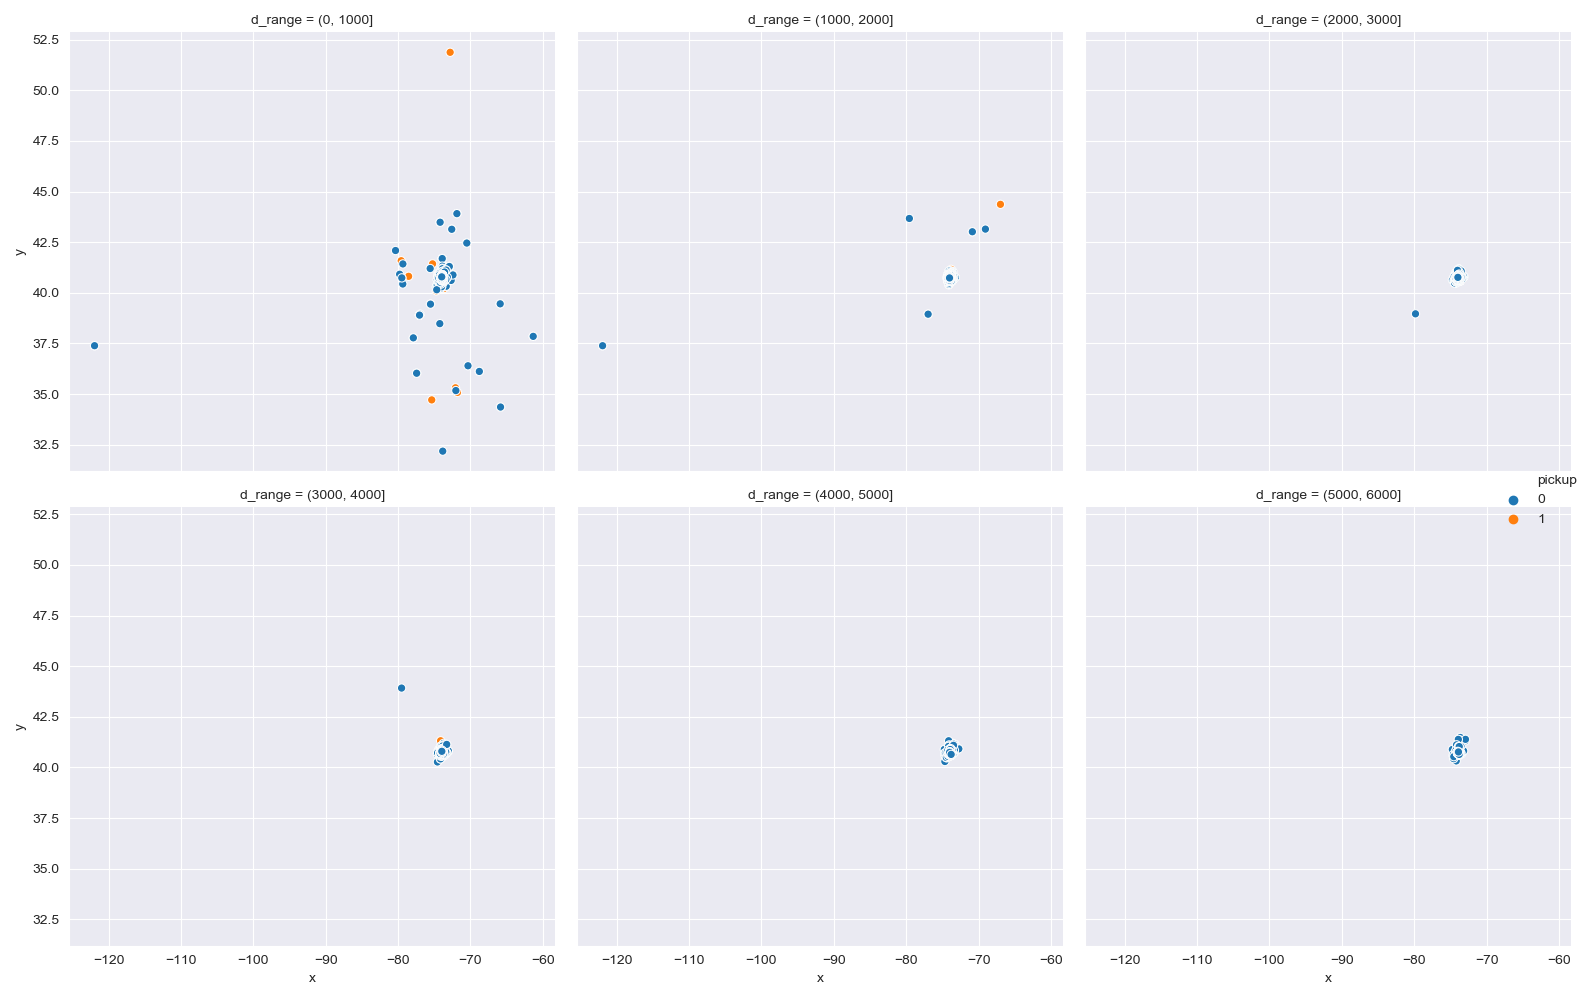
\includegraphics[width=0.8\textwidth]{figures2/duration_geo.eps}
    \caption{Faraway position affact on duration plot}
    \label{fig:geographic-duration}
  \end{figure}
\end{slide}

\begin{slide}{Clean Geographic}
  \begin{itemize}
    \item Keep data which stay in range [0.001\%, 99.999\%] of original data
  \end{itemize}
  \begin{figure}[h]
    \centering
    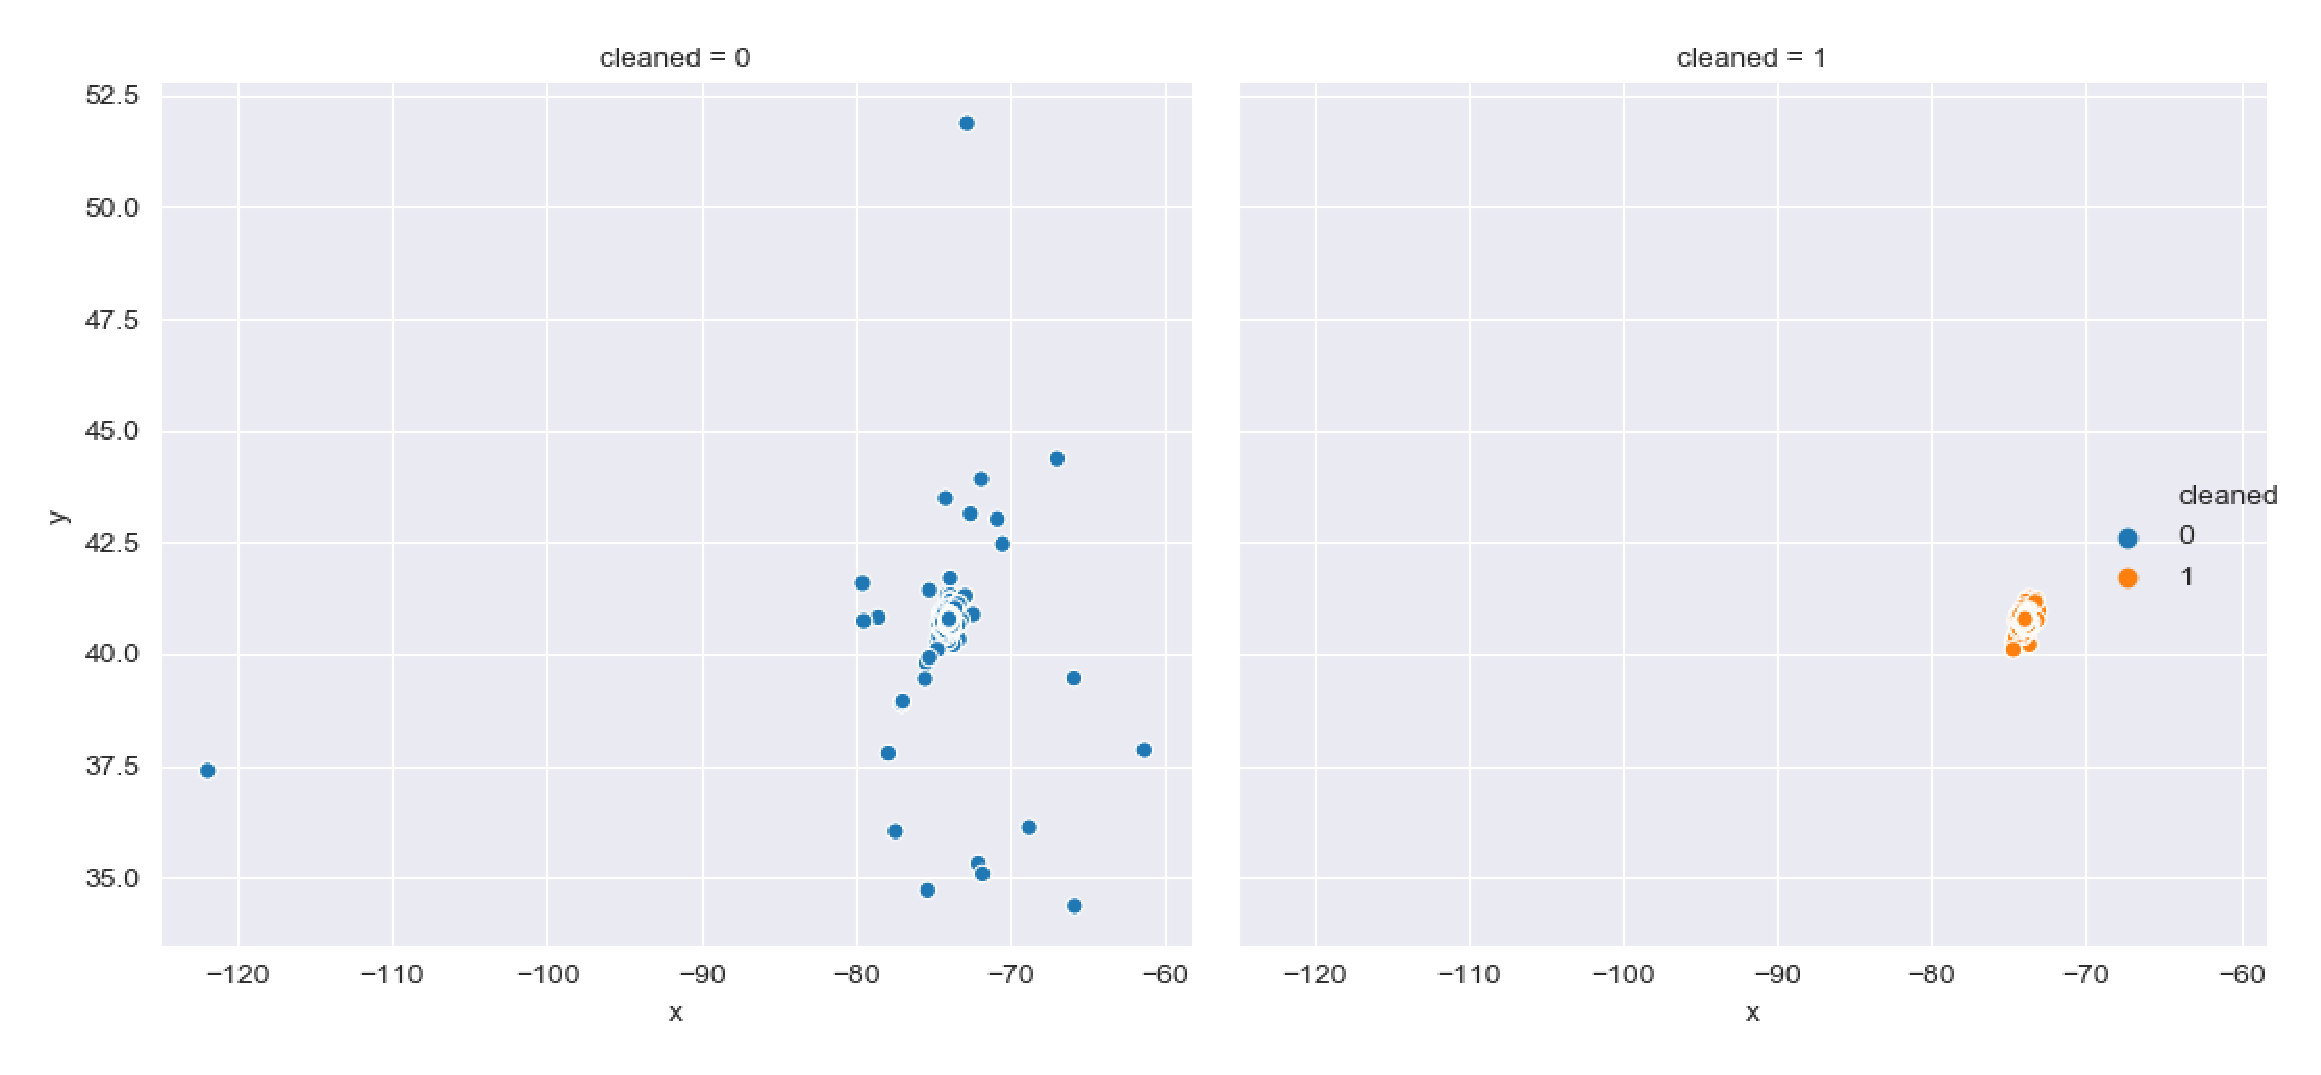
\includegraphics[width=0.8\textwidth]{figures2/cleaned_position.eps}
    \caption{Origin vs cleaned locations plot (pickup)}
    \label{fig:cleaning-geographic}
  \end{figure}
\end{slide}

\begin{slide}{Cleaned Geographic}
  \begin{itemize}
    \item Pickup vs dropoff positions (cleaned)
  \end{itemize}
  \begin{figure}[h]
    \centering
    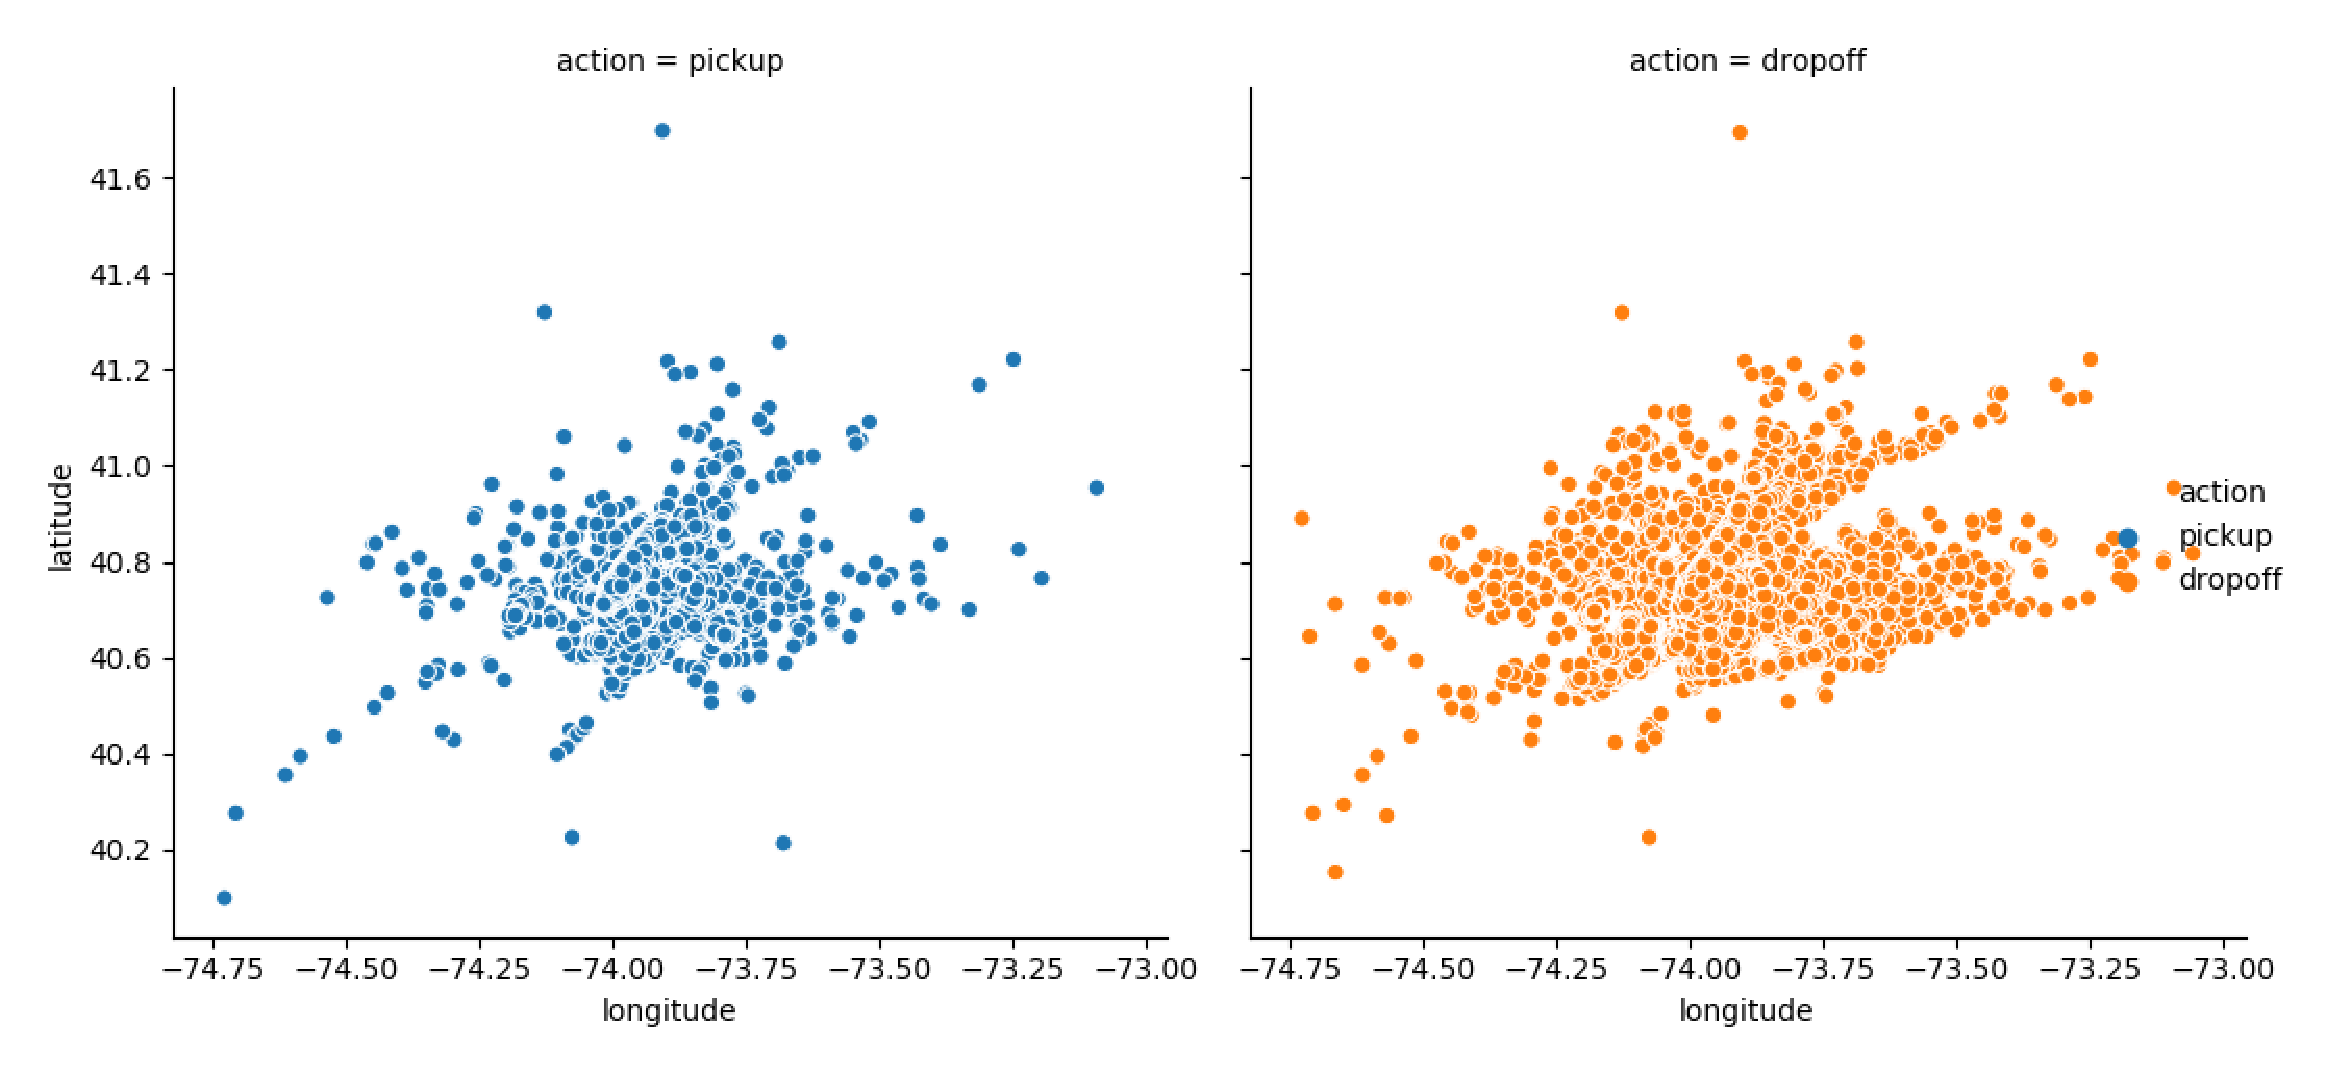
\includegraphics[width=0.8\textwidth]{figures2/pd.eps}
    \caption{Pickup vs dropoff locations plot (cleaned)}
    \label{fig:clean-geographic}
  \end{figure}
\end{slide}


\begin{slide}{Vendor Id}
  \begin{itemize}
    \item Count plot
  \end{itemize}
  \begin{figure}[h]
    \centering
    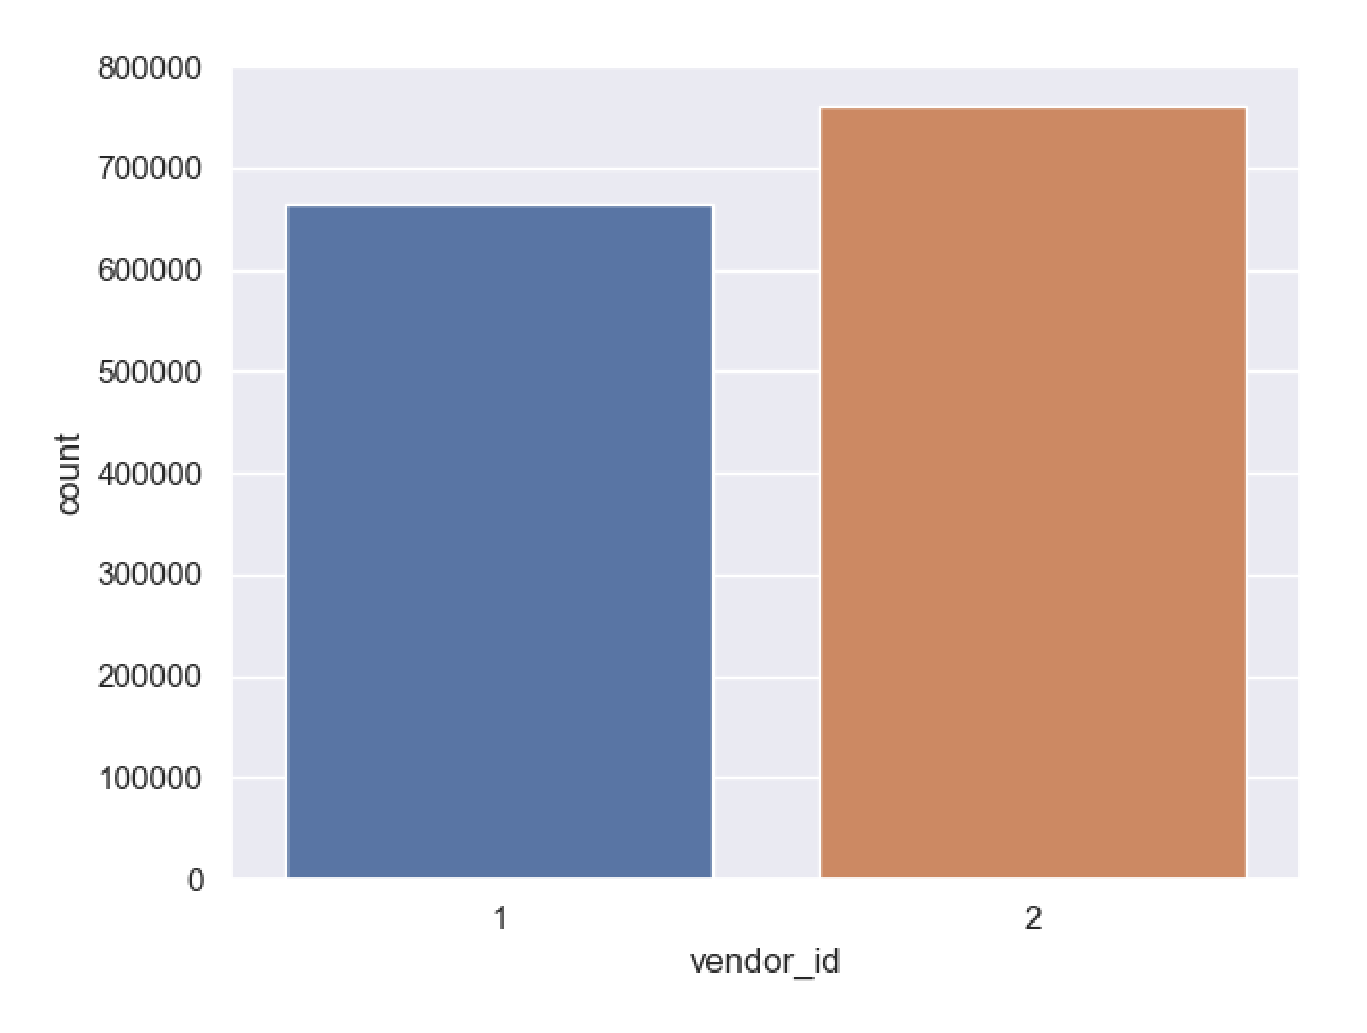
\includegraphics[width=0.6\textwidth]{figures2/vendor_id.eps}
    \caption{Count by vendor id}
    \label{fig:vendor-id}
  \end{figure}
\end{slide}

\begin{slide}{Vendor Id - Passenger count}
  \begin{itemize}
    \item Count plot splited by passenger count
  \end{itemize}
  \begin{figure}[h]
    \centering
    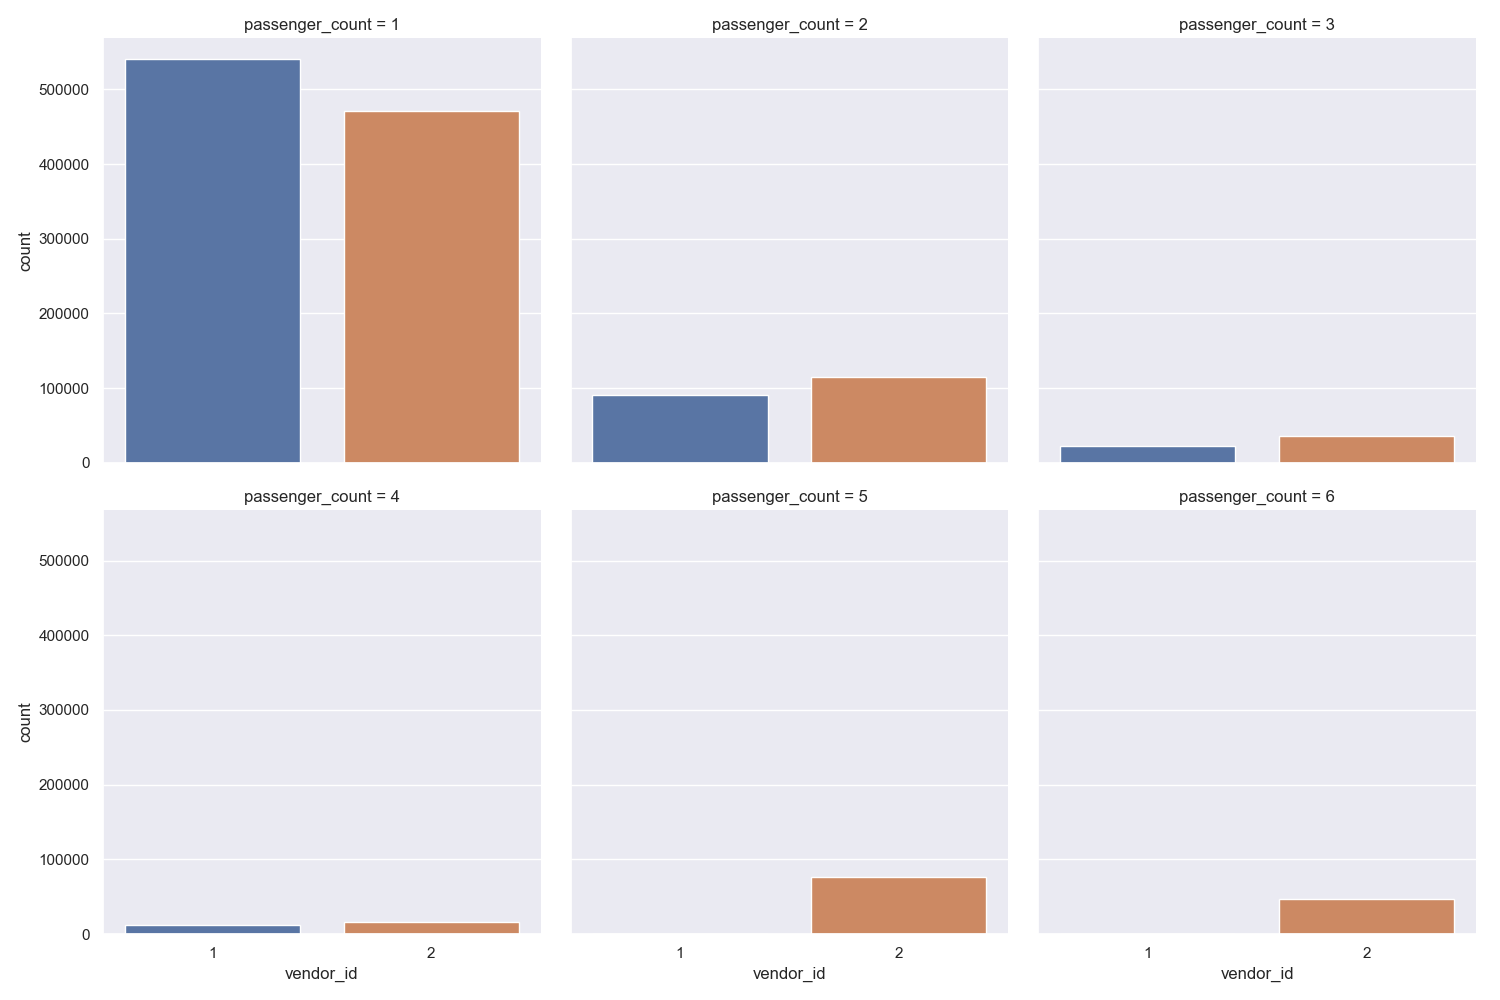
\includegraphics[width=0.7\textwidth]{figures2/vendor_id_count.eps}
    \caption{Count by vendor id and passenger id}
    \label{fig:vendor-id-passenger-count}
  \end{figure}
\end{slide}

\begin{slide}{Vendor Id - Geographic location}
  \begin{itemize}
    \item Count plot splited by geographic location
  \end{itemize}
  \begin{figure}[h]
    \centering
    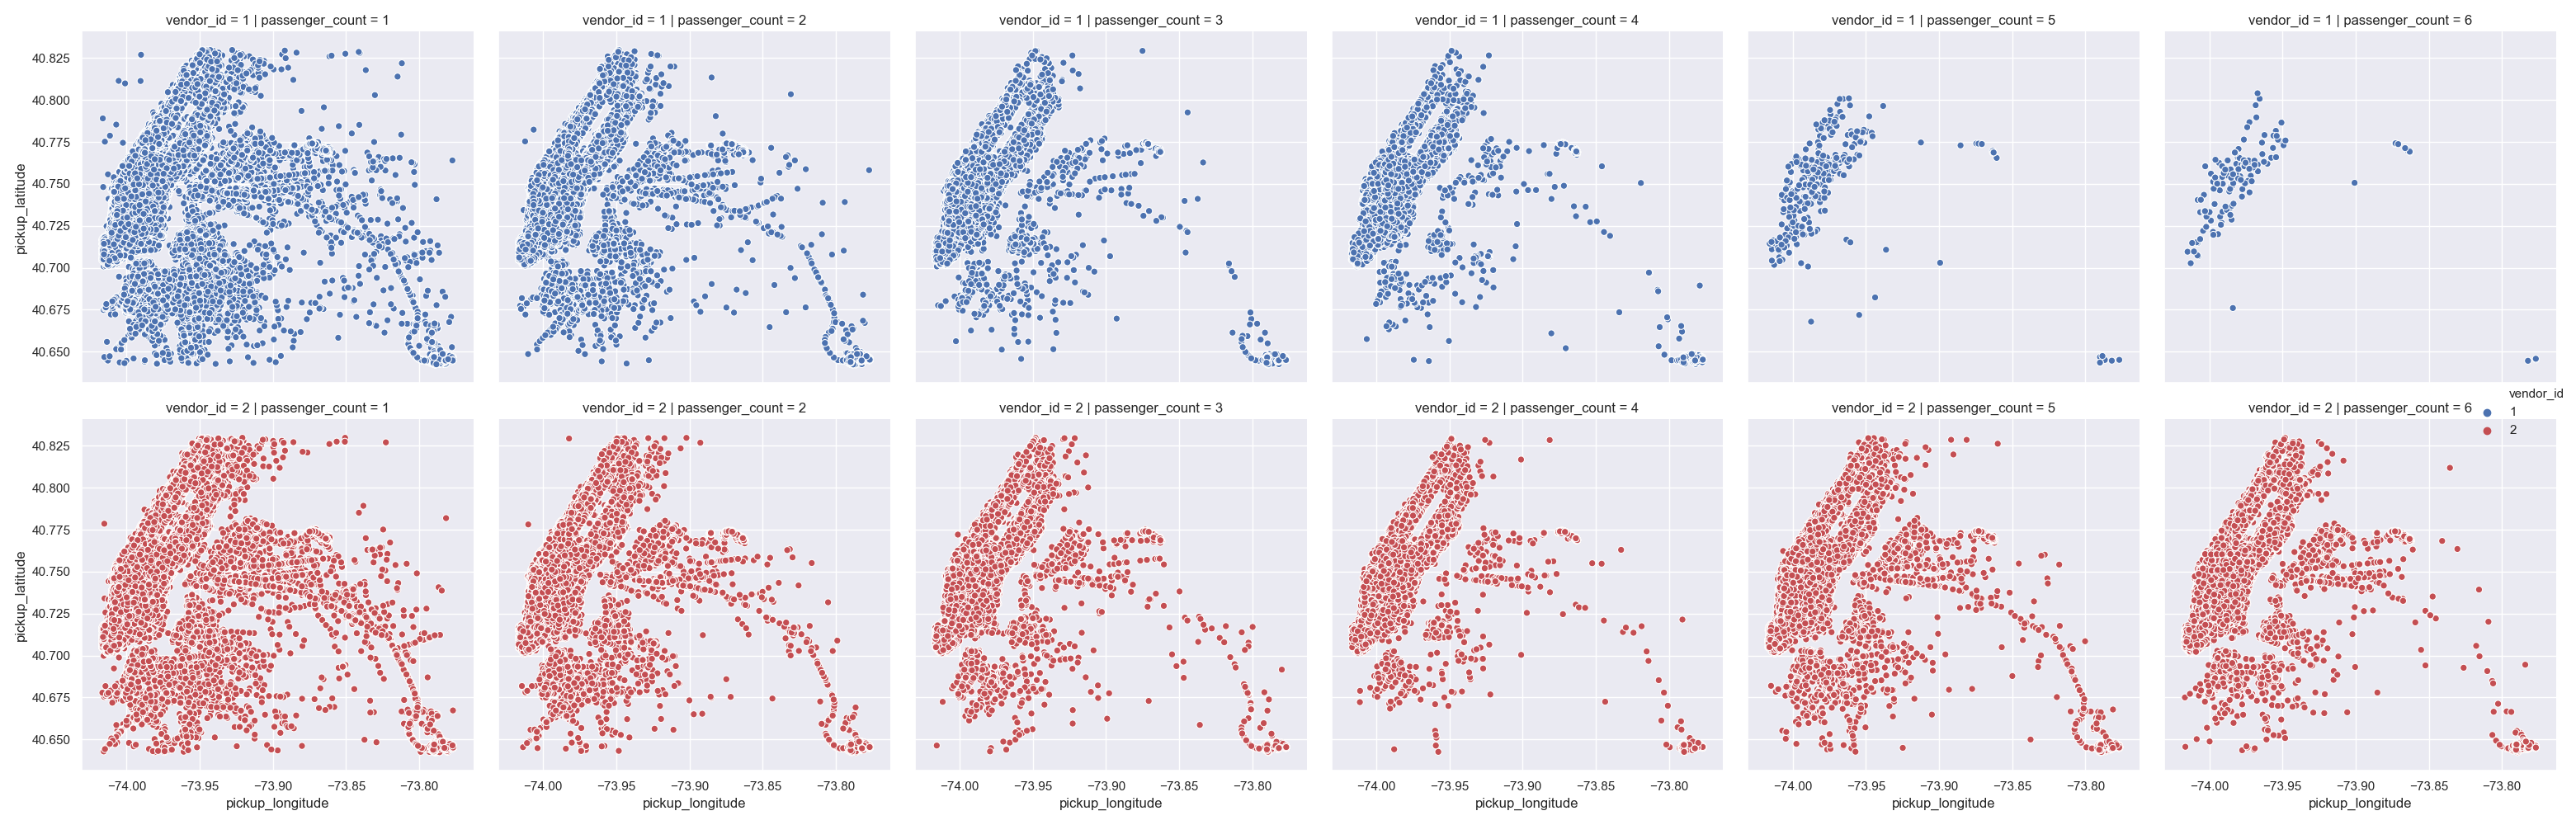
\includegraphics[width=1.0\textwidth]{figures2/vendor_geo.eps}
    \caption{Vendor id in geographic}
    \label{fig:categories-picture}
  \end{figure}
\end{slide}


\begin{slide}{Passenger count}
  \begin{itemize}
    \item Count trips by passenger count in train/test dataset
    \item Both proportions for passengers count are: 0.709, 0.144, 0.041, 0.019, 0.054, 0.033, 0.000, 0.000, 0.000 \pause
    \begin{figure}[h]
      \begin{minipage}[t]{0.4\linewidth}
        \centering
        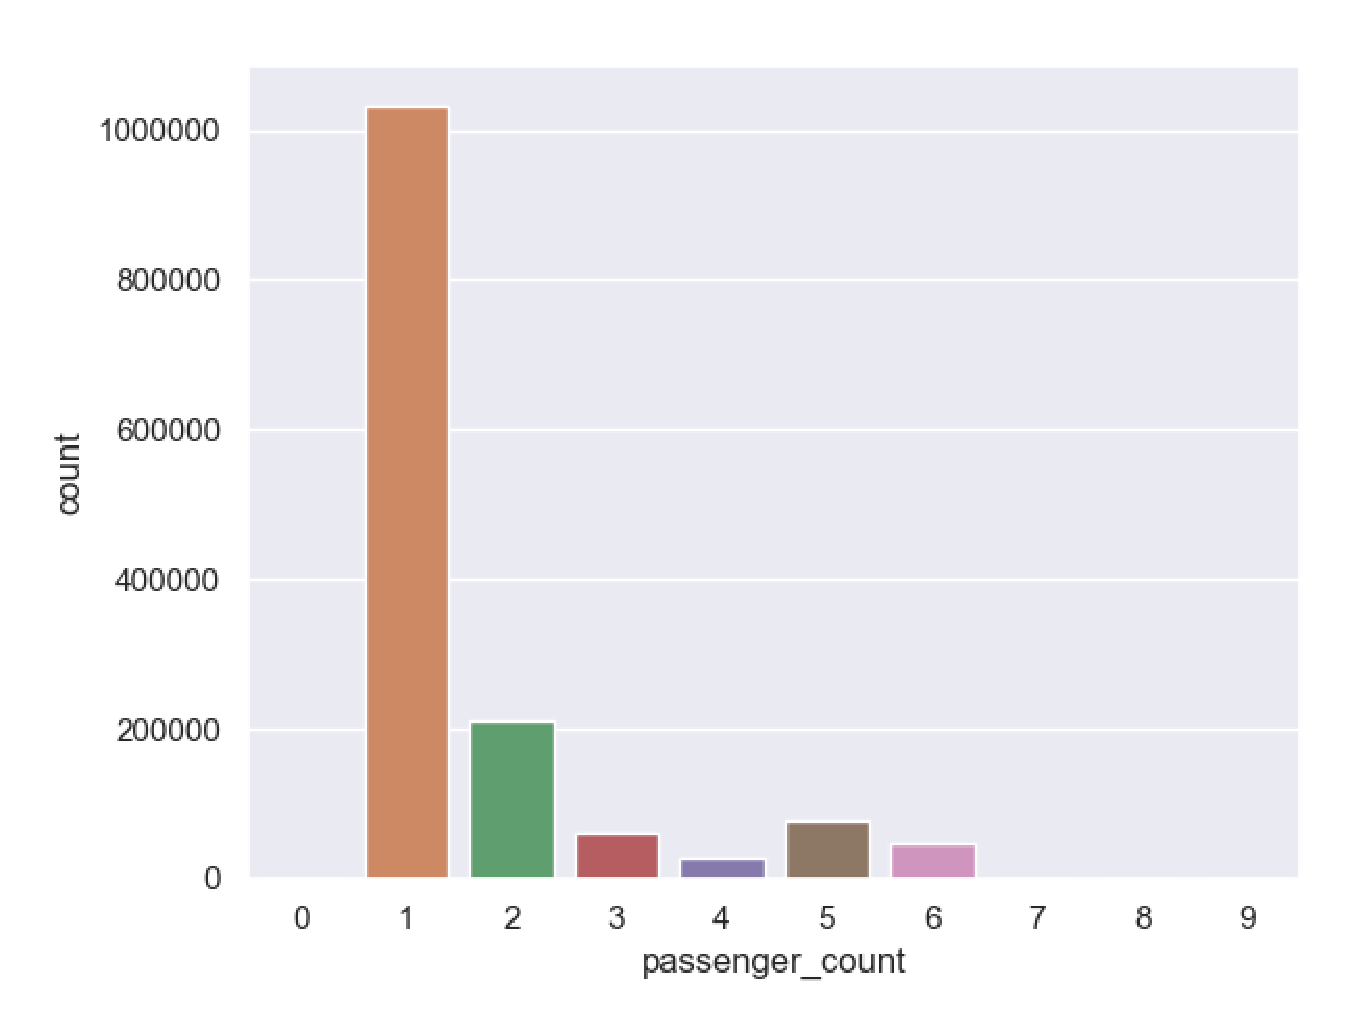
\includegraphics[width=1.0\textwidth]{figures2/passenger_count_train.eps}
        \caption{Count trips in train dataset by passenger count}
        \label{fig:count-by-passenger-count}
      \end{minipage}
      \pause
      \hfill
      \begin{minipage}[t]{0.4\linewidth}
        \centering
        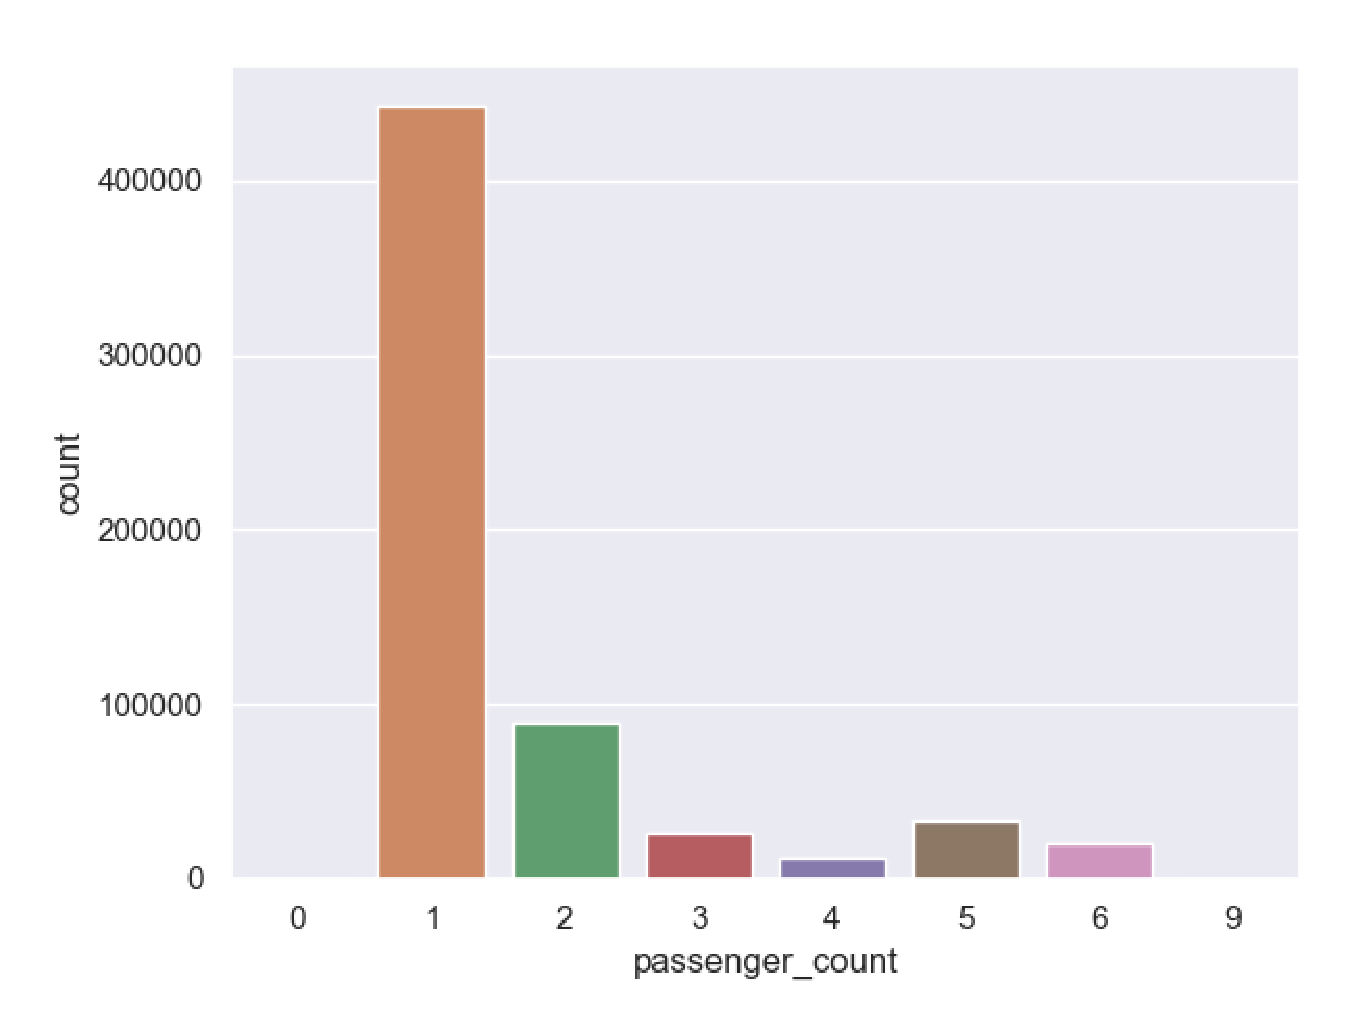
\includegraphics[width=1.0\textwidth]{figures2/passenger_count_test.eps}
        \caption{Count trips in test dataset by passenger count}
        \label{fig:count-by-passenger-count-test}
      \end{minipage} 
    \end{figure}
  \end{itemize}
\end{slide}


\begin{slide}{Store and fwd}
  \begin{itemize}
    \item Store and fwd count plot
    \begin{figure}[h]
      \centering
      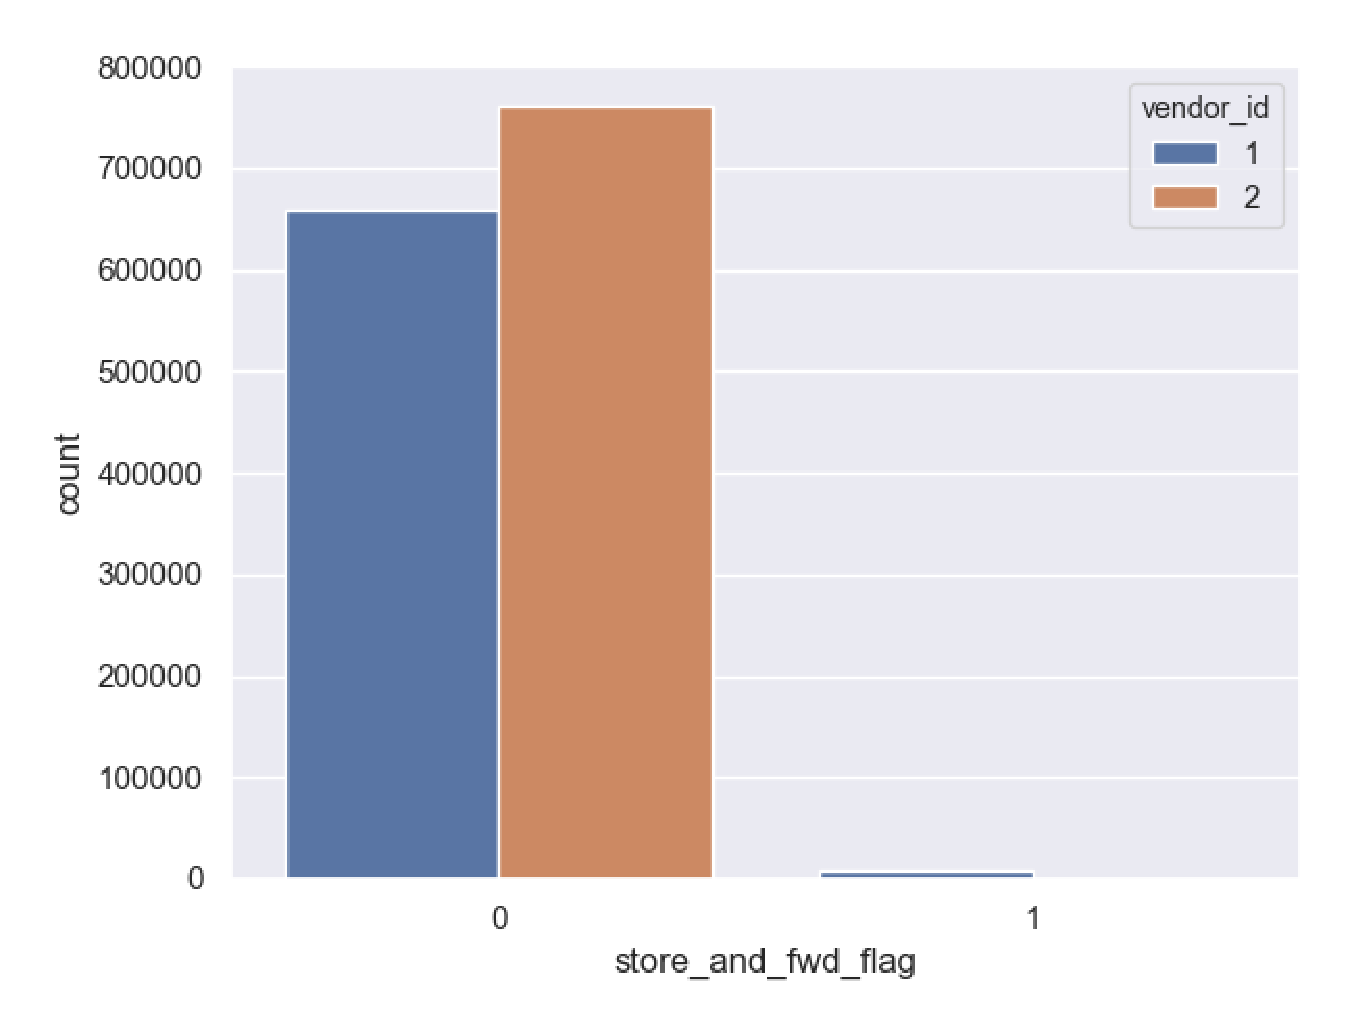
\includegraphics[width=0.6\textwidth]{figures2/store_and_fwd_flag.eps}
      \caption{Store and fwd count plot}
      \label{fig:store-and-fwd}
    \end{figure}
  \end{itemize}
\end{slide}

\begin{slide}{Timestamps} month_count
  \begin{itemize}
    \item Count by different time frame in one day
    \begin{figure}[h]
      \begin{minipage}[t]{0.3\linewidth}
        \centering
        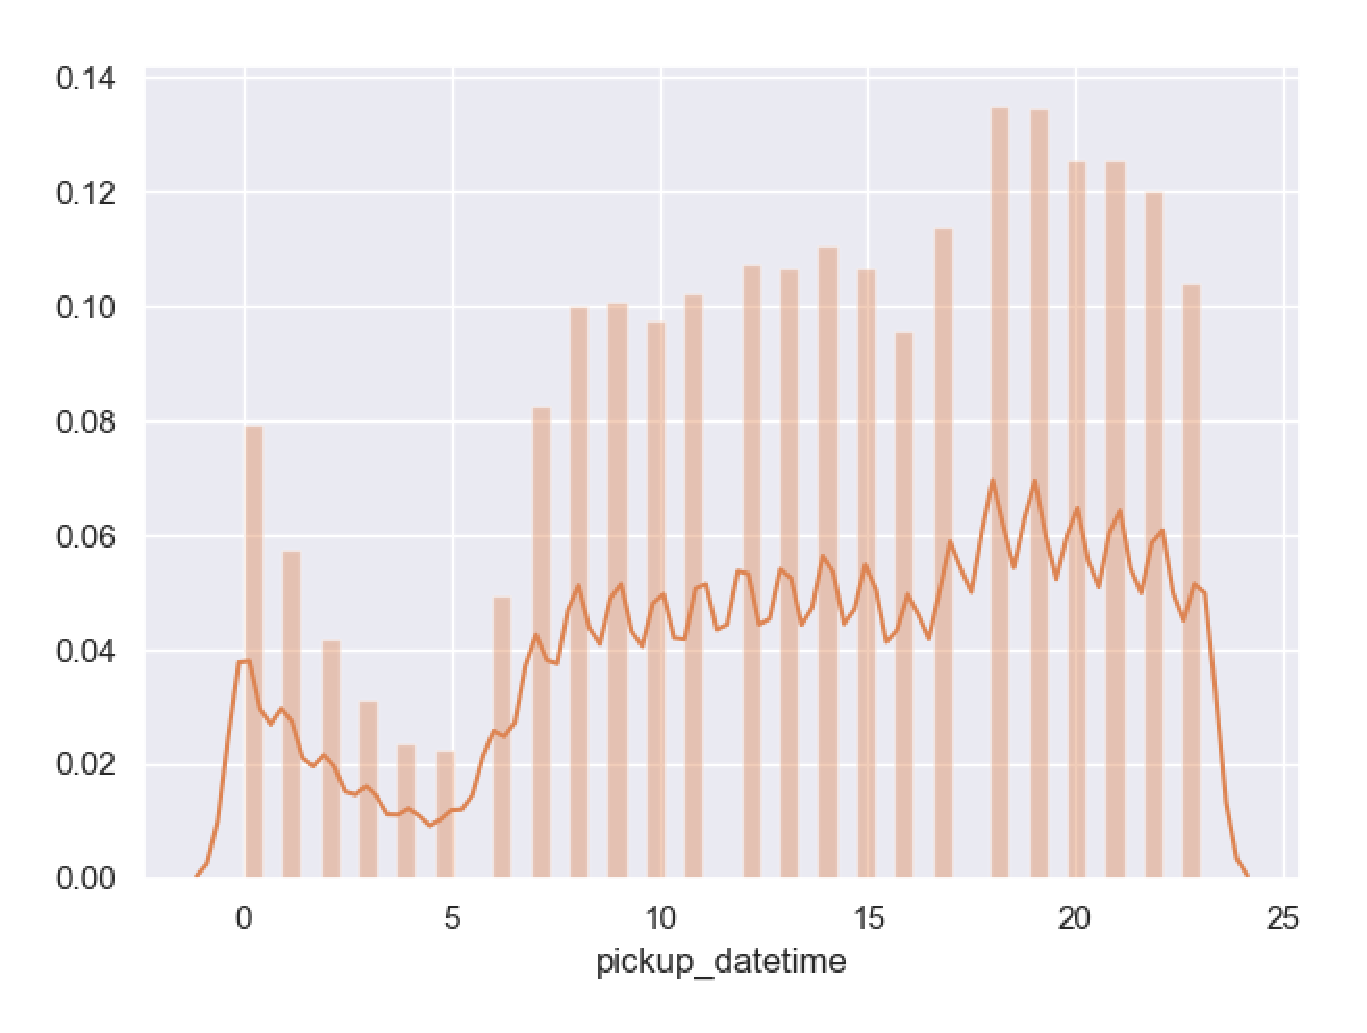
\includegraphics[width=1.0\textwidth]{figures2/pickup_hour_distribution.eps}
        \caption{Trip count by time frame in one day}
        \label{fig:timestamps-picture}
      \end{minipage} 
      \pause
      \hfill
      \begin{minipage}[t]{0.6\linewidth}
        \centering
        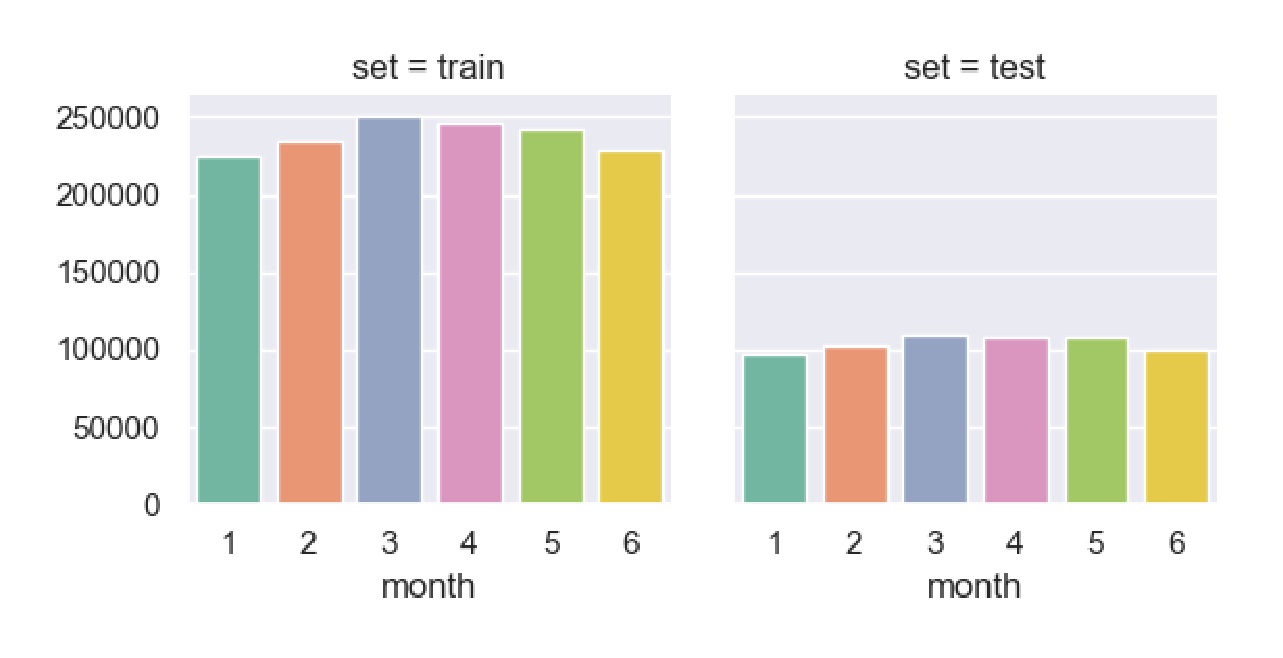
\includegraphics[width=1.0\textwidth]{figures2/month_count.eps}
        \caption{Trip count by month}
        \label{fig:count-by-passenger-count-test}
      \end{minipage} 
    \end{figure}

    \begin{figure}[h]
      
    \end{figure}
  \end{itemize}
\end{slide}

\begin{slide}{Trip Duration}
  \begin{itemize}
    \item Trip duration
    \begin{figure}[h]
      \centering
      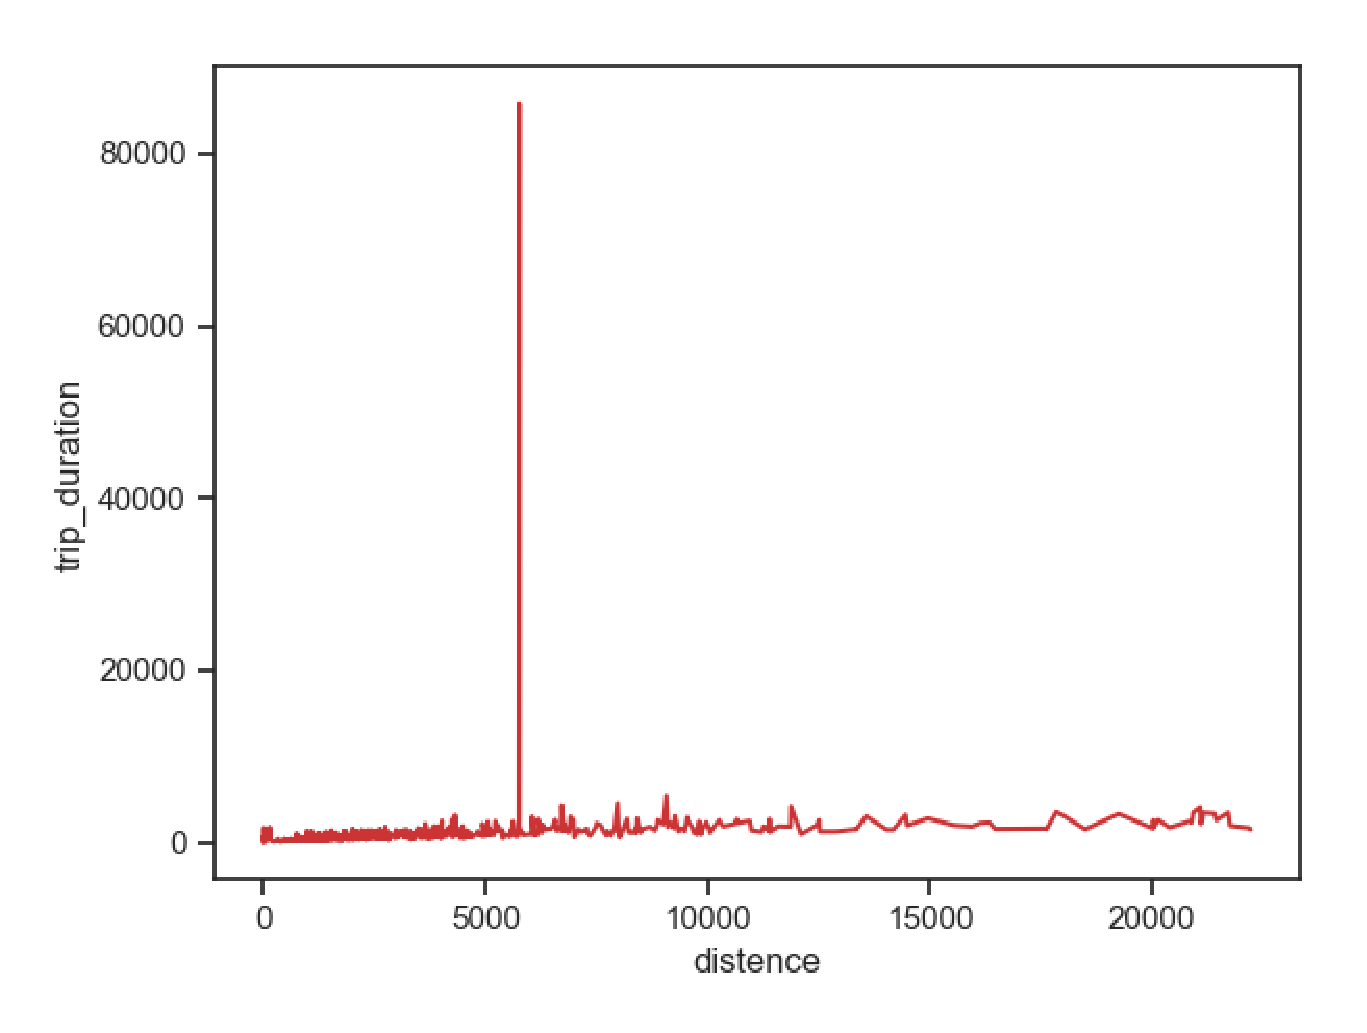
\includegraphics[width=0.6\textwidth]{figures2/distence_trip_duration_relation.eps}
      \caption{Relation between distance and Trip duration}
      \label{fig:trip-duration-distribution-picture}
    \end{figure}
  \end{itemize}
\end{slide}


\section{Data Preprocess}

\begin{slide}[toc=,bm=]{Overview of Data Preprocess}
  \tableofcontents[content=currentsection,type=0]
\end{slide}

\begin{slide}{Clean}
  \begin{itemize}
    \item Exclude out outliers in geographic \pause
    \item Exclude out outliers by passenger count \pause
    \item Exclude out outliers in trip duration (labels) \pause
  \end{itemize}
\end{slide}

\begin{slide}{Append}
  \begin{itemize}
    \item Distance, manhattan distance and haversine distance \pause
    \item Weekday, weekend, month, day, hour \pause
    \item Exclude out outliers in trip duration (labels) \pause
    \item Area
    \begin{figure}[h]
      \centering
      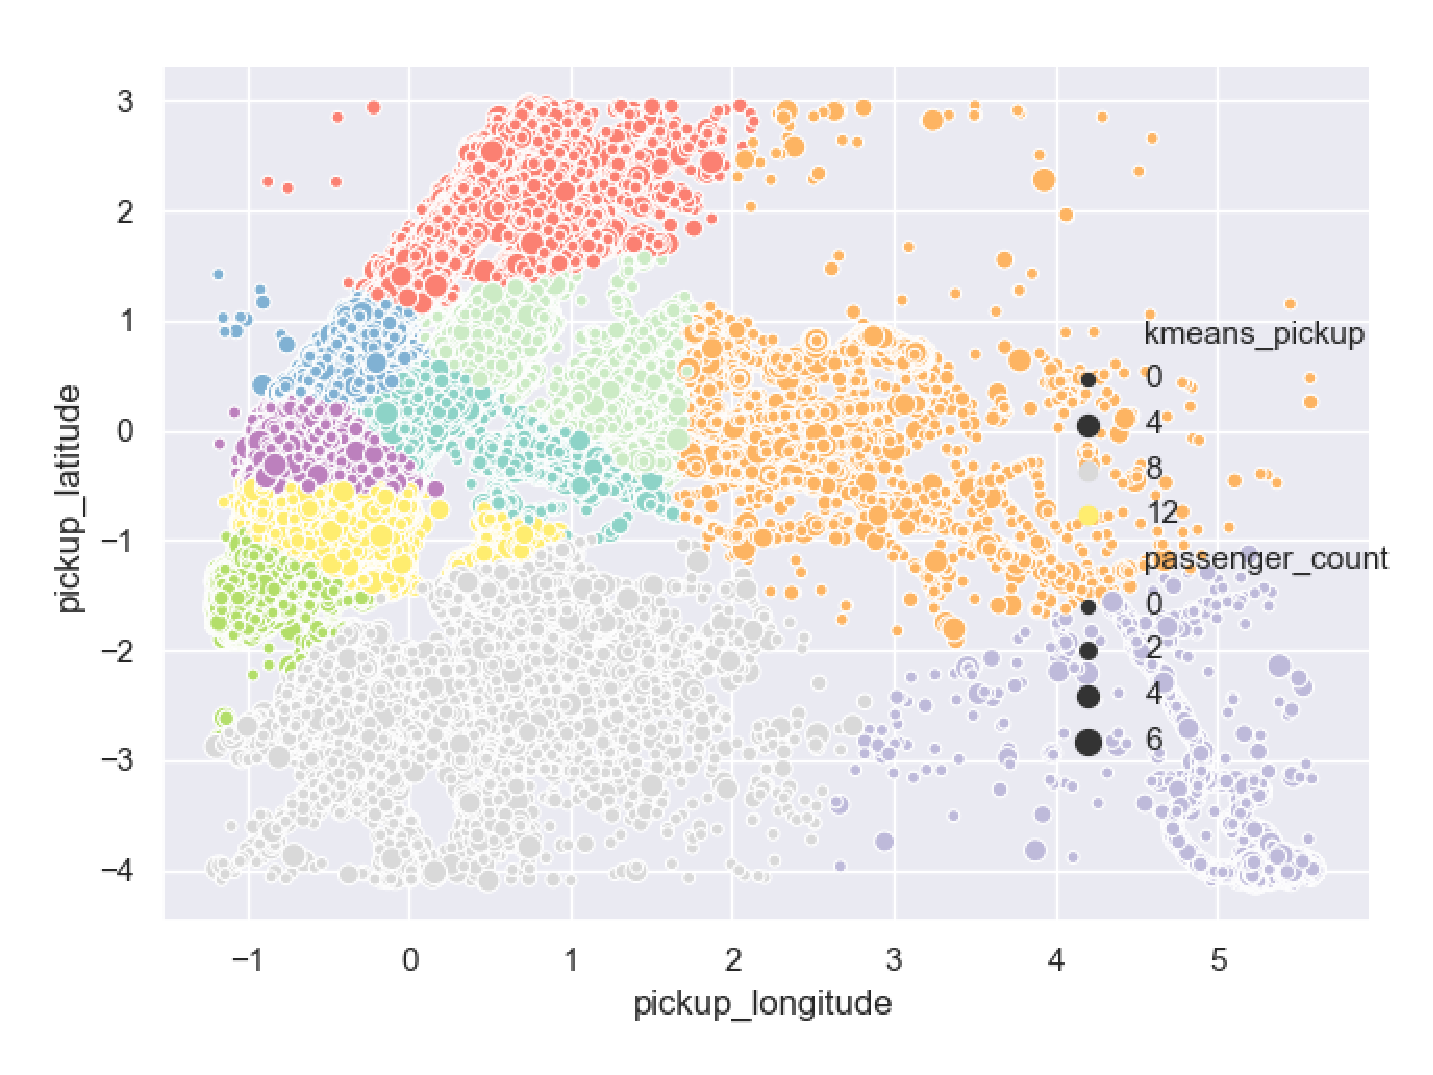
\includegraphics[width=0.5\textwidth]{figures2/area.eps}
      \caption{Split into different areas}
      \label{fig:area-geo}
    \end{figure}
  \end{itemize}
\end{slide}


\begin{slide}{Normalization}
  \begin{itemize}
    \item Standard Normalization 
    $$
    z = \frac{X-\mu}{\delta}
    $$
    \pause
    \item MinMax Scaler
    $$
    z = \frac{X-min}{max-min}
    $$
    \pause
    \item Use MinMax Scaler for distance, timestamps, passenger count, vendor id \pause
    \item Use Standard Normalization Scaler for the others \pause
  \end{itemize}
\end{slide}


\section{Model Selection}

\begin{slide}[toc=,bm=]{Overview of Model Selection}
  \tableofcontents[content=currentsection,type=0]
\end{slide}

\begin{slide}{RandomForestRegresser}
  \begin{itemize}
    \item Composed of multi classification and regression Trees \pause
    \item No need for features selection \pause
    \item Simple, stable
  \end{itemize}
\end{slide}

\begin{slide}{Xgboost}
  \begin{itemize}
    \item Weighting on examples
    \item Support sampling on features \pause
  \end{itemize}
\end{slide}

\begin{slide}{LightGBM}
  \begin{itemize}
    \item Optimal Split for Categorical Features \pause
    \item Leaf-wise (Best-first) Tree Growth \pause
    \item Faster training speed and higher efficiency \pause
    \item Lower memory usage \pause
    \item Better accuracy \pause
  \end{itemize}
\end{slide}


\section{Experiment}

\begin{slide}[toc=,bm=]{Overview of Experiment}
  \tableofcontents[content=currentsection,type=0]
\end{slide}

\begin{slide}{First shot}
  \begin{itemize}
    \item RandomForestRegresser
    \begin{itemize}
      \item Without cleaning or new feature
      \item Run with default parameters
      \item 5-fold Cross Validataion
      \item Score of train/validation/submission: 0.53484/0.53213/0.55944
    \end{itemize}
  \end{itemize}
\end{slide}


\begin{slide}{Try with operations on features}
  \begin{itemize}
    \item RandomForestRegresser
    \begin{itemize}
      \item With cleaning, new-feature and normalization
      \item GridSearchCV in n_estimators and max_depth
      \item 5-fold Cross Validataion
      \item Score of train/validation/submission: 0.43956/0.44046/0.44709
      \item std in train/validation: 0.00052/0.00064 
      \begin{figure}[h]
        \begin{minipage}[t]{0.4\linewidth}
          \centering
          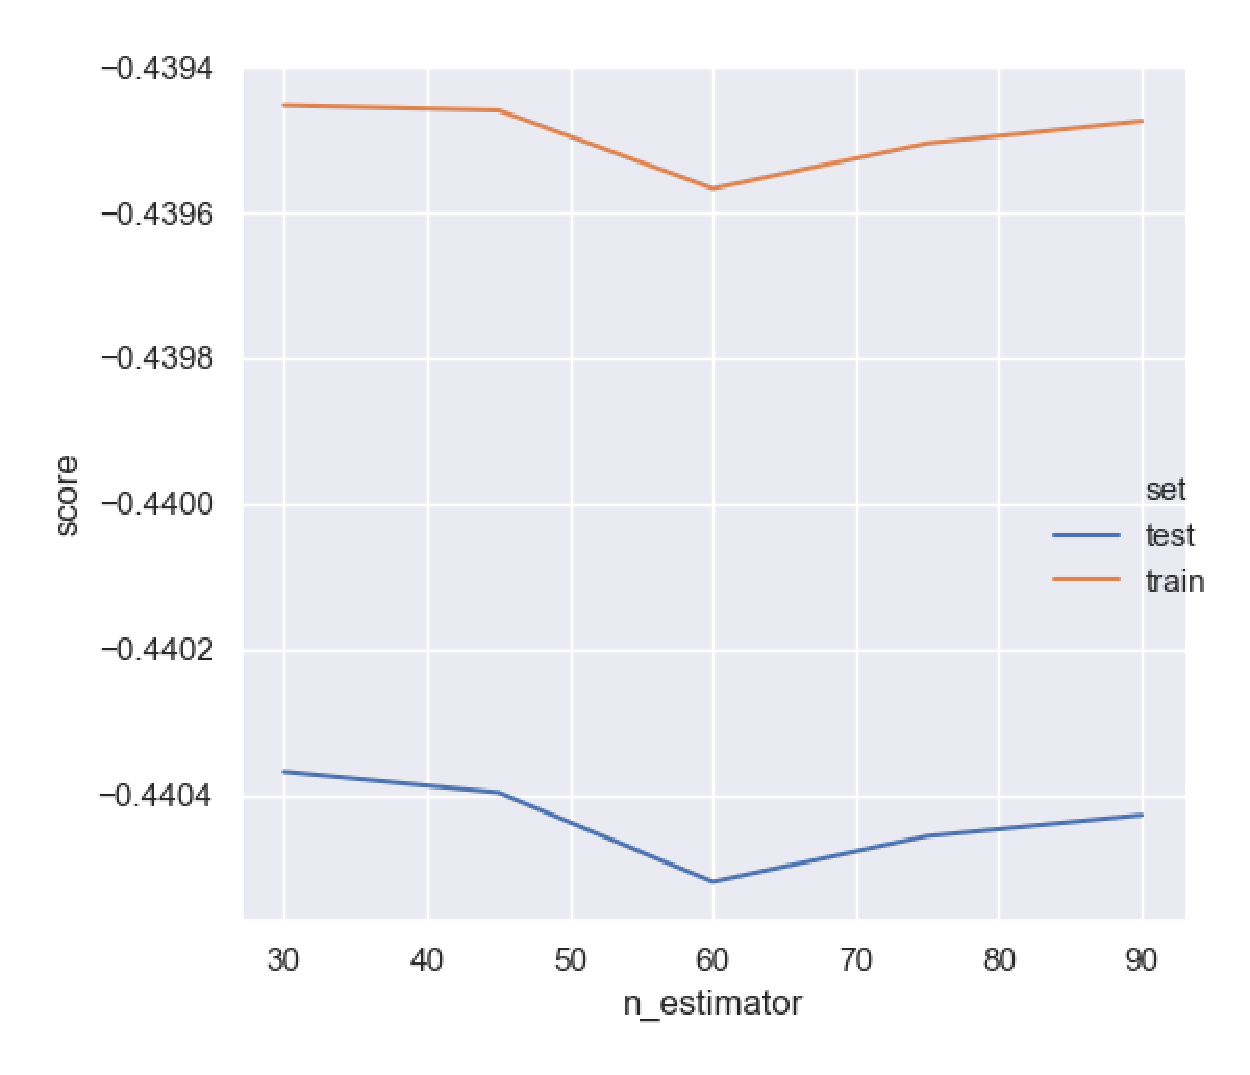
\includegraphics[width=1.0\textwidth]{figures2/rfr-estimator.eps}
          \caption{Rfr scores var different n estimators}
          \label{fig:rfr-estimators}
        \end{minipage}
        \hfill
        \begin{minipage}[t]{0.4\linewidth}
          \centering
          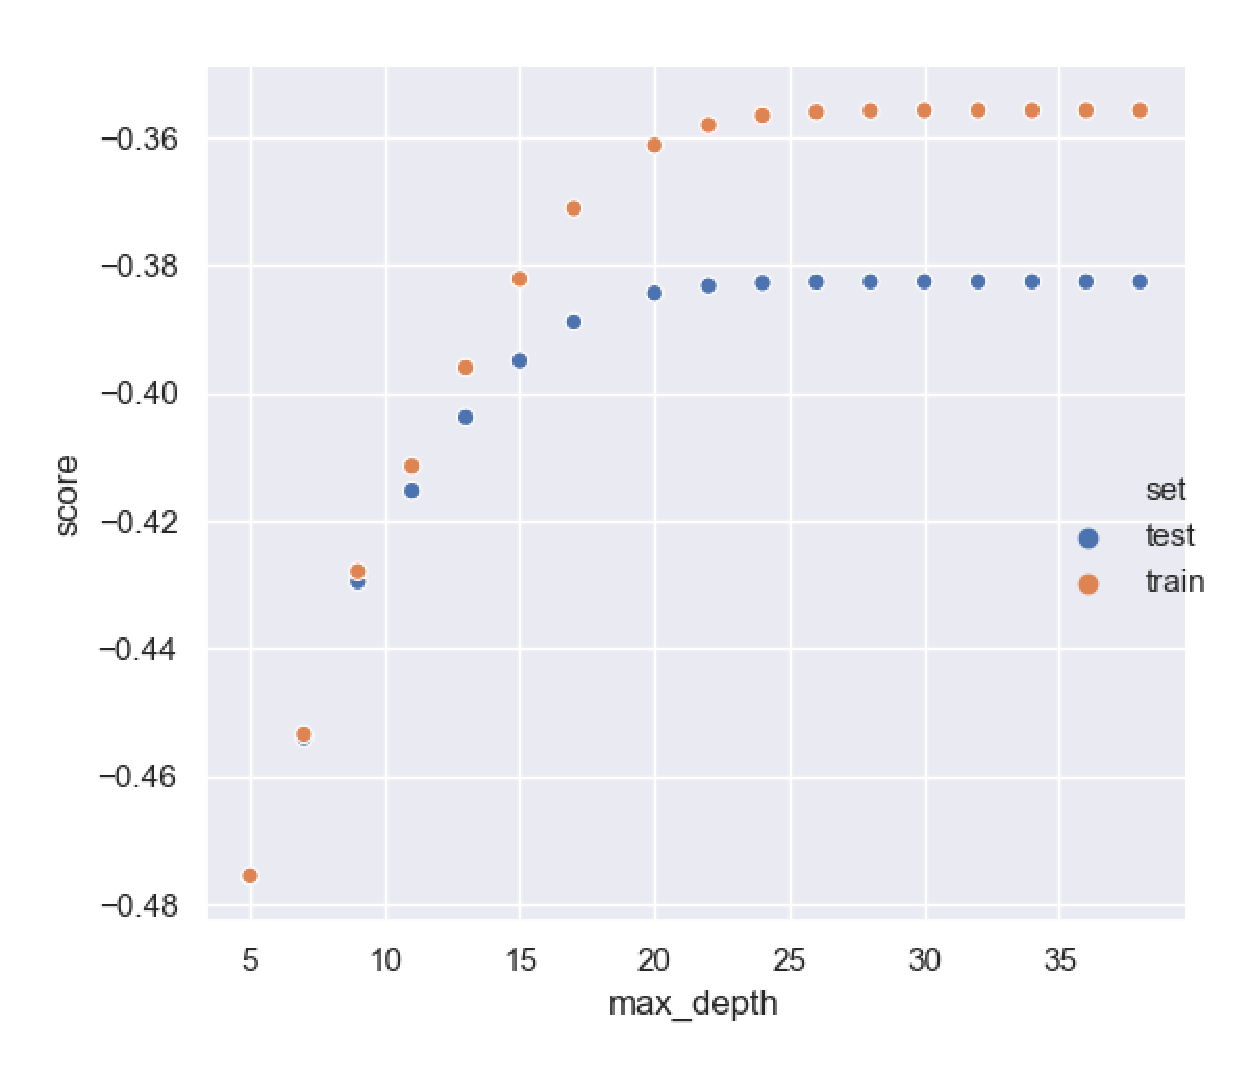
\includegraphics[width=1.0\textwidth]{figures2/max_depth_score.eps}
          \caption{pictures labeled as 1}
          \label{fig:rfr-max-depth}
        \end{minipage} 
      \end{figure}
    \end{itemize}
  \end{itemize}
\end{slide}

\begin{slide}{Try with new model}
  \begin{itemize}
    \item LightGBM
    \begin{itemize}
      \item With cleaning, new-feature and normalization
      \item GridSearch in max_depth, n_estimators, 
      \item 5-fold Cross Validataion \pause
      \item Score of submission: 0.420020
      \item std in train/validation: 0.00111/0.00078 \pause 
      \begin{figure}[h]
        \begin{minipage}[t]{0.4\linewidth}
          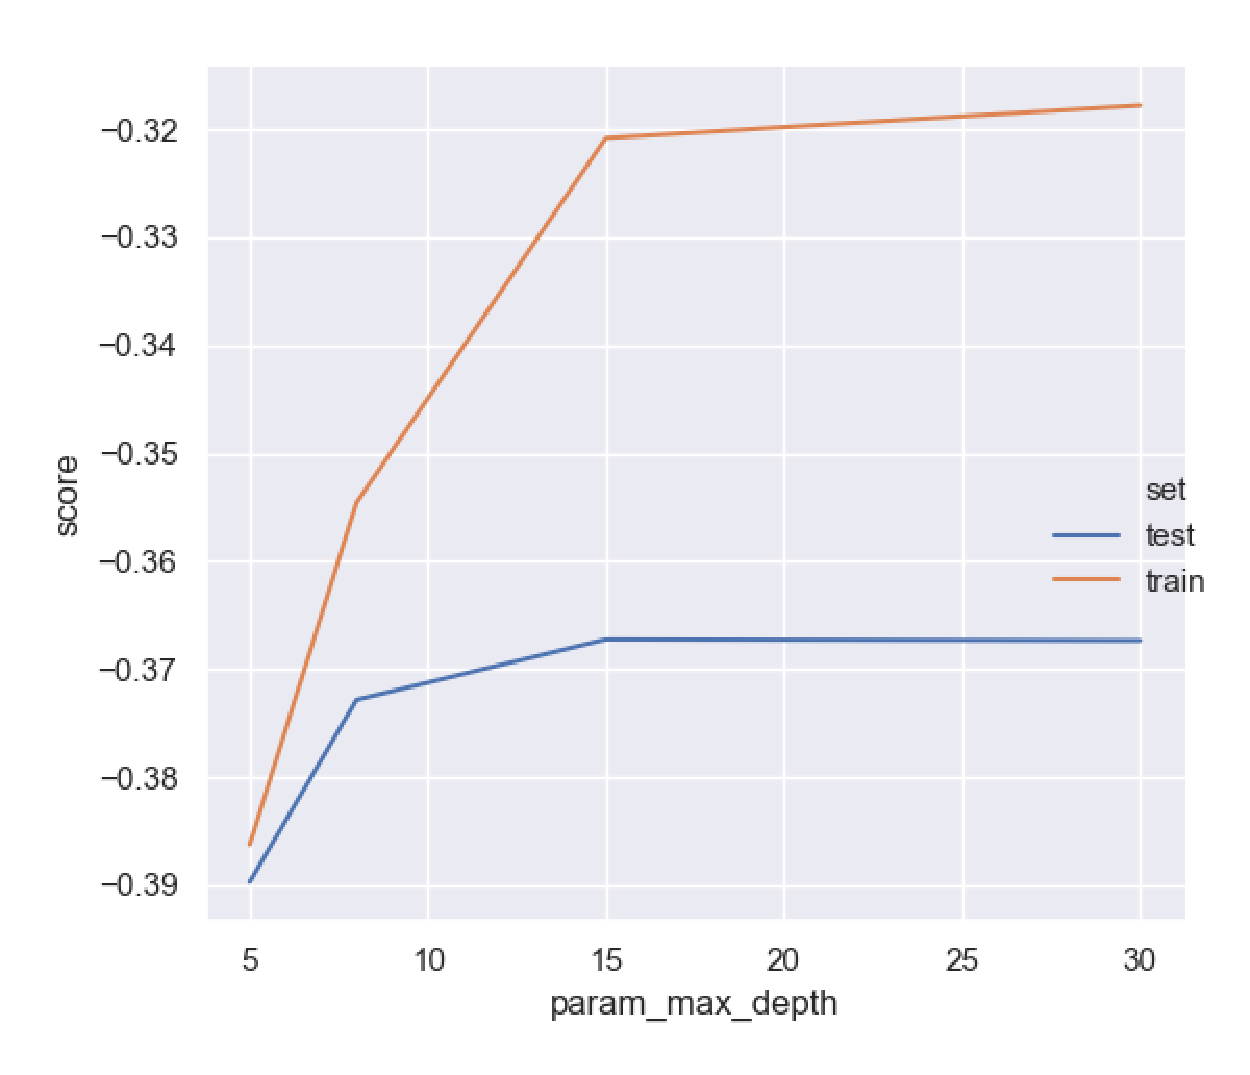
\includegraphics[width=1.0\textwidth]{figures2/lgb_max_depth.eps}
          \caption{Lgb scores var in maxdepth}
          \label{fig:lgb-max-depth}
        \end{minipage}
        \hfill
        \begin{minipage}[t]{0.4\linewidth}
          \centering
          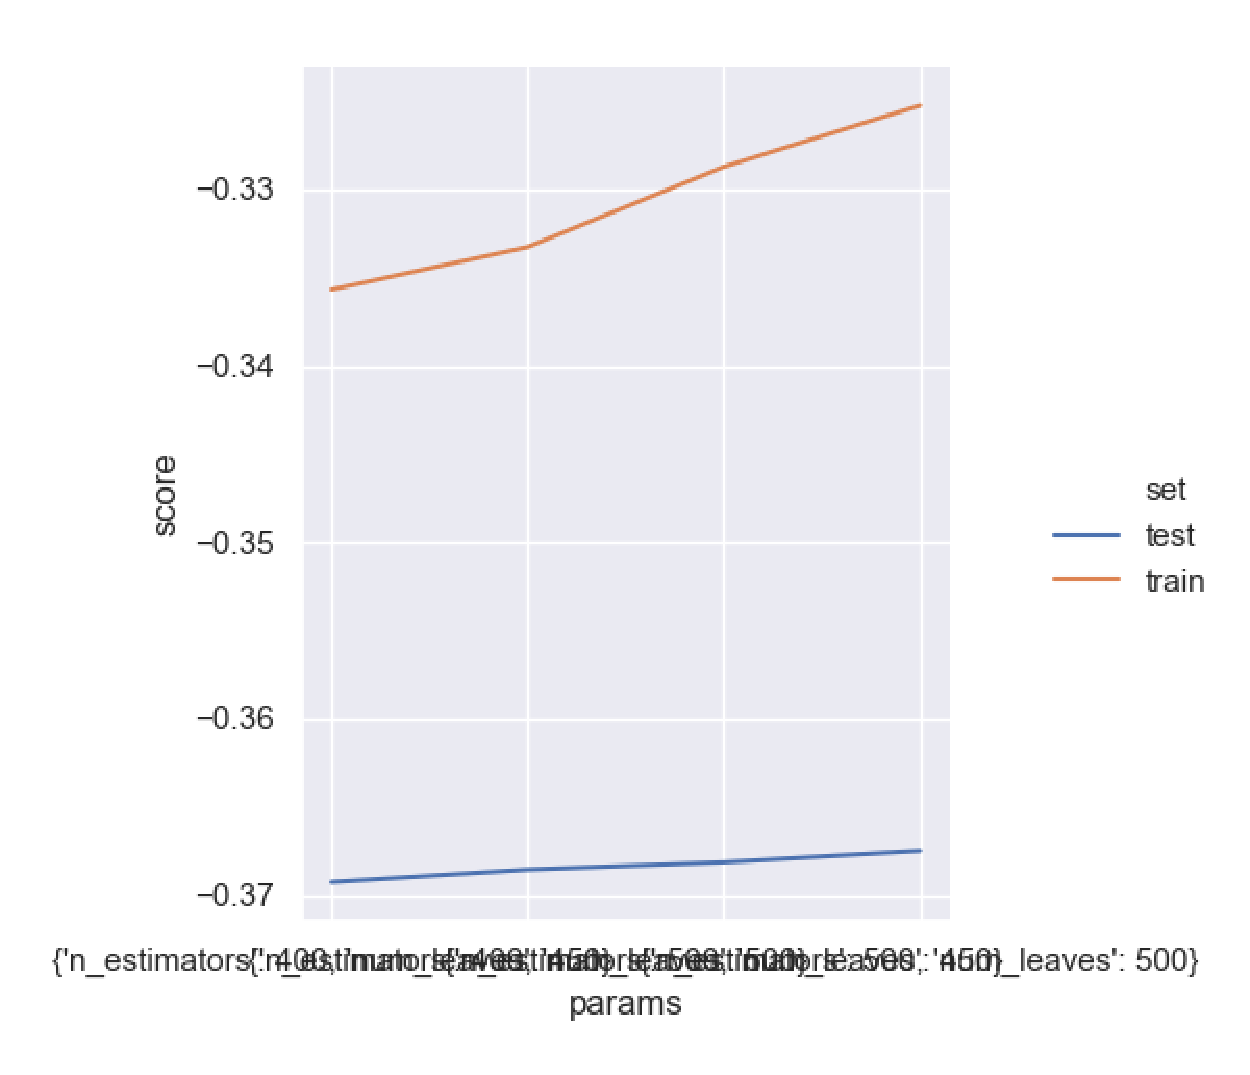
\includegraphics[width=1.0\textwidth]{figures2/lgb_n_leaves.eps}
          \caption{Lgb scores var in n estimators and min leaves}
          \label{fig:lgb-n-leaves}
        \end{minipage} 
      \end{figure}
    \end{itemize}
  \end{itemize}
\end{slide}

\begin{slide}{Try with different boosting type of LightGBM model}
  \begin{itemize}
    \item LightGBM
    \begin{itemize}
      \item With cleaning, new-feature and normalization
      \item GridSearch in boosting type: 'default', 'dart', 'goss', 'rf'
      \item 5-fold Cross Validataion \pause
      \item Worse than the default
    \end{itemize}
  \end{itemize}
\end{slide}


\begin{slide}{Rank of Competition}
  \begin{itemize}
    \item Score: 0.41895
    \item Rank: 545/1207
  \end{itemize}
  \begin{figure}[h]
    \centering
    
\includegraphics[width=0.8\textwidth]{figures2/score.eps}
    \caption{Result of the best submission}
    \label{fig:result-of-best-submission}
  \end{figure} 
\end{slide}


\section{Summary}

\begin{slide}{Thanks}
  \begin{itemize}
    \item Thanks for listening~
  \end{itemize}
\end{slide}

% \begin{slide}{References (1)}
% \bibliographystyle{plain}
% \nobibliography{YourBib}
% \bibentry{someone1}
% \bibentry{someone2}
% \end{slide}
% \begin{slide}{References (2)}
% \bibentry{someone3}
% \end{slide}

% \begin{slide}{Slide}
% \cite{someone}
% \end{slide}
% 
% \begin{slide}{References}
% \bibliographystyle{plain}
% % \bibliography{YourBib}
% \end{slide}

\end{document}

\endinput
